% adapted by WS from SSR's Word document and from the 5-part series at
% https://www.overleaf.com/learn/latex/How_to_Write_a_Thesis_in_LaTeX_(Part_1):_Basic_Structure
% reviewed by MAM

\documentclass[12pt,twoside]{report}

\usepackage[titletoc]{appendix} % for adding appendix to TOC
\usepackage[backend=biber]{biblatex}  % reference management
\usepackage{geometry}  % better margins and margin control
\usepackage{graphicx}  % to include figures
\usepackage{hyperref}  % internal and external links
\usepackage[utf8]{inputenc}  % support for non-ASCII characters
\usepackage[T1]{fontenc}  % proper encoding for special characters
\usepackage{listings}  % typset code
\usepackage{outlines}  % easy nesting of lists
\usepackage{tabularx}  % more control over table column width
\usepackage{titlesec}  % customize chapter title 
\usepackage{upquote}  % prevent mishandling of single quotes in listings
\usepackage{amsmath}
\usepackage{amssymb}  % for \mathbb
\usepackage{float}
\usepackage{xcolor}  % for colors
\usepackage{colortbl}  % for \cellcolor in tables
\usepackage{booktabs}  % for \addlinespace in tables
% TODO: Customize the appearance of hyperref links using \hypersetup
% See https://en.wikibooks.org/wiki/LaTeX/Hyperlinks#Customization

% Custom format of chapter title.
\titleformat{\chapter}[hang]{\bf\huge}{\thechapter.}{2pc}{}


% Reduce spacing around sections
\titlespacing*{\chapter}{0pt}{-30pt}{20pt}
\titlespacing*{\section}{0pt}{12pt}{6pt}
\titlespacing*{\subsection}{0pt}{10pt}{4pt}
\titlespacing*{\subsubsection}{0pt}{8pt}{2pt}

% Separate folder for images named 'images'.
\graphicspath{ {images/} }

% Separate file for references
\addbibresource{references.bib}

% Replace with your title
\title{Quadruped Locomotion in Rough Terrain and Confined Environments}

% Allow recalling document title
% from https://tex.stackexchange.com/a/15806/44301
\makeatletter\let\Title\@title\makeatother  

\begin{document}

\begin{titlepage}
  
  \newgeometry{top=100pt,bottom=75pt}   
  \begin{center}
    \vfill
    \textbf{\Huge \Title}
    \bigskip

    {\large Kaavish Report\\
      presented to the academic faculty\\
      by\\\bigskip
      % replace with your name and HU ID
      \begin{tabular}{ll}
        Hania Kashif & hk08454\\
        Raahim Hashmi & rh08461\\
        Syed Zuhair Abbas Rizvi & sr07889\\
      \end{tabular}
    }\\\vfill
    
\includegraphics[width=.4\textwidth]{Logo.png}\\
    {\large In partial fulfillment of the requirements for\\
      \textit{Bachelor of Science}\\
      Computer Science\\\medskip
      \textbf{Dhanani School of Science and Engineering}\\\medskip
      Habib University\\\smallskip
      Spring 2026
    }\\\vfill
    Copyright {\scriptsize \textcopyright} 2019 Habib University
  \end{center}
  \restoregeometry
\end{titlepage}

%%% Local Variables:
%%% mode: latex
%%% TeX-master: "report"
%%% End:
  % title page.
\include{approval}  % approval page.

\chapter*{Dedication}
Our work is dedicated to those that don’t bend, don’t water it down, don’t try to make it logical, don’t edit their own souls according to the fashion; rather, they follow their most intense obsessions mercilessly.

(Quote taken from Franz Kafka)

\chapter*{Acknowledgements}
There are far too many wonderful people to thank here that made this project not just possible but victorious. Some of these, however, deserve special mention, so here they are.

We begin with the titular protagonist: the \textit{Leegit Robot}, also known as the Lynxmotion T-Hex 3DoF Hexapod. Our gratitude is insurmountable towards it for existing in the first place to set our FYP into motion. Its resilience throughout our countless experiments, failed and successful, will be remembered dearly. We hope that whoever inherits it for future work will take it to grander heights.

Next, we would like to thank our supervisors Dr. Saleha Raza and Dr. Basit Memon for their unwavering support and guidance, amid uncountable difficulties particularly during inception, throughout Kaavish. It was because of their insights and feedback that we stayed focused as we journeyed through the trials and tribulations of our capstone. Additionally, we are also grateful to our co-supervisor Mr. Tabsheer Ali Askari for his devotion to planning and assessing progress as well as managing the testbed developments. 

Beyond that, we must mention our university friends for sticking around and being fun to talk to about their own capstones, wonderful and not-so-wonderful coursework, plans after graduation, and sundries. Similarly, we extend our gratitude towards the many brilliant faculty from DSSE and AHSS both that, with their teachings within and outside the classroom from algorithms to art, inspired us to become who we are. Furthermore, we cannot forget the patience and moral support of our families during times of distress, discombobulation, and disenchantment. And, to all the lovely folk of the world who produced art, music, film, games, and literature that remind us of what it means to live life for beyond university and work, thank you.  

Lastly, to the reader, who may be a student looking for inspiration on their own FYP, know that the capstone will be, quite literally, an experience to remember for the rest of your \textbf{life.}  

\chapter*{Abstract}
Mobile robots are widely used for inspection, exploration, and search and rescue missions. Legged robots, in contrast to wheeled robots, have the added benefit of legged locomotion which allows them to tackle a wide variety of different terrains that a wheeled robot cannot. Caves, abandoned tunnels, and collapsed buildings are examples of environments that consist of such terrain. Using an existing hobby-grade quadruped robot kit, we sought to make it capable of traversing rough terrain and navigate through confined spaces. We created a complete simulation package for the robot, which was previously missing. We augmented the hardware kit with mounts for our compute modules and sensors to obtain feedback required for robust locomotion. For locomotion in rough terrain, we tested classical control techniques, learning-based approaches, and evolutionary algorithms. To allow the robot to navigate through confined spaces, like crawling under an obstacle or squeezing through a narrow gap, we used a depth camera for perceiving the immediate terrain and deciding on a posture that was used to constrain the locomotion algorithms to ensure the robot moved with a height and width that did not collide with the environment. Thanks to our simulation package, we were able to rapidly test our algorithms, without the added hassle and risk of testing on hardware. 

% The following are automatically populated by LaTeX \chapter, \section and related, \figure, and \table.
\tableofcontents
\listoffigures
\listoftables

\chapter{Introduction}
\label{chap:intro}
\section{Problem Statement}

Mobile robots have widespread applications in industrial inspection, terrestrial and extraterrestrial exploration, and search and rescue missions. Wheeled or tracked systems are the most prevalent types of mobile robots that are being used for these tasks \cite{IntroductionAutonomousMobile}. Such robots typically adapt to changes in terrain through passive mechanical feedback \cite{belterAdaptiveMotionPlanning2016} and require a continuous path of support with minimal obstructions \cite{raibertLeggedRobotsThat1986} which restricts the kind of environments such systems can tackle to a minority of Earth's total landmass \cite{raibertBigDogRoughTerrainQuadruped2008}. Several critical environments, such as caves, forests, collapsed buildings, etc, pose challenges to these systems or render them entirely unusable. At the same time, these environments' terrain pose little challenge to animals, particularly ones that use legs for locomotion. Inspired from such animals, legged robots are an alternative category of mobile robots that are highly attractive due to their ability to traverse challenging terrain. Unlike wheeled or tracked systems that require a long patch of unobstructed terrain, legged robots only require isolated footholds to be unobstructed, greatly increasing their versatility in highly cluttered environments and rough terrain. Furthermore, they can climb over obstacles or squeeze through tight gaps by changing their morphology, similar to legged animals.

The current state-of-the-art robots such as Boston Dynamics' Spot \cite{Spot}, ANYBotics' ANYmal \cite{hutterANYmalHighlyMobile2016}, and Unitree's Go Series quadrupeds are used for assisting or even replacing humans in a variety of tasks due to their impressive locomotion capabilities \cite{SpotRescue, SpotRobotAssists, boumanAutonomousSpotLongRange2020, NovoNordiskExplores, gehringANYmalFieldSolving2021, tranzattoCERBERUSAutonomousLegged2022, hoellerANYmalParkourLearning2023, UnitreeFirefightingRobots2025}. Such high-end systems cost thousands of dollars \cite{kimPADWQDesignControl2021} due to expensive actuators, sensors, and compute modules.

We define, therefore, the problem statement of this capstone project as follows: 

\textit{How can we make a low-cost quadruped capable of traversing rough terrain in a purely proprioceptive manner? Furthermore, if we simulate a massless depth camera on the robot, how can we make the robot capable of navigating confined spaces using perception-based locomotion?}

\section{Proposed Solution}

We use a hobbyist robot kit, a Lynxmotion T-Hex 3DoF Hexapod repurposed into a quadruped, in order to demonstrate an inexpensive yet effective alternative for such robots. Our vision is that the robot, with teleoperation, would be able to handle varied rough terrain in real life while extending its behavior to perceive close environments using a camera and adapt its posture to minimize collisions while maintaining consistent and safe locomotion. Aside from proving that our locomotion pipeline is capable of working in even hobby-grade robots with adequate results, our proposed pipeline remains agile, versatile, and capable of further research and specialization for use cases such as search-and-rescue, cave exploration, and sundries.

\section{Intended User}

Our robotics systems's intended primary users are: researchers on robotics, academic developers, and operators looking for teleoperable platforms capable of exploring rough, confined environments such as subterranean caves, collapsed buildings, mountains, hazardous zones in construction, and so on.

\section{Project Gantt Chart and Deliverables}


\subsection{Kaavish I}
\begin{enumerate}
    \item Adopting the existing hardware and making the robot walk on flat ground. This includes:
    \begin{itemize}
        \item Re-assembling the robot to ensure proper orientation of motors. The robot was assembled by someone from EE 2023, and we cannot simply trust that it was assembled properly as improper assembly can result in having invalid commands to the motors causing irreparable damage
        \item Interfacing the motor controller with a Raspberry Pi 4. The current microcontroller for the robot is outdated and is not suitable for the tasks we intend to execute on the robot. As such, we will replace it with a Raspberry Pi 4 and interface that with the existing motor controller
        % \item Statistical analysis of the motors for better repeatability. The servo motors used in the legs do not have a readable angle output; for precise control, we would need to model the inaccuracy of each servo reaching a commanded position and incorporate that in our control strategies
        % \item Building a battery for the robot as per power requirements, keeping in mind future additions 
        \item Integrating all the hardware all together and implementing a basic gait. This gait does not need to be able to deal with rough terrain, it will simply be obtained from the kinematic model of the robot and is intended to make the robot walk on flat ground
    \end{itemize}
    \item Building the simulation model for the robot as well as the simulation environment. This includes:
    \begin{itemize}
        \item Identifying a suitable simulation environment. To ensure accurate simulation of locomotion strategies, a high fidelity physics engine like MuJoCo could be suitable; however, other considerations include integration with ROS and the ability to import custom models and environments
        \item Making a 3D model of the robot. The Lynxmotion website provides \texttt{sldprt} files that can be converted to \texttt{stp} files that can then be modified if needed and imported into any simulation software
        \item Identifying the parameters for the lava tubes terrain and scaling them down appropriately. 
        \item Making a simulation environment for testing. This can be handcrafted based on the parameters identified, but procedural random generation will allow for the robot to be extensively tested in simulation with better generalization and there is some recent work that suggests this could be possible \cite{garciaPLUMEProceduralLayer2025}
    \end{itemize}
    \item Extensive literature review of locomotion strategies, with some selected to be tested for the robot. The strategies will be selected based on a number of considerations, including the incorporation of feedback (open-loop vs closed-loop), novelty, and proven success. We will ensure that the selected strategies stretch across a number of paradigms, e.g. evolutionary algorithms, model-based RL, model-free RL etc.
    \item Literature review and initial implementation of multi-elevation mapping techniques. This includes:
\begin{itemize}
    \item Studying robot-centric mapping approaches and their application to confined space navigation \cite{buchananWalkingPostureAdaptation2019, mikiLearningRobustPerceptive2022}
    \item Implementing basic distance sensor data processing for multi-elevation map generation
    \item Developing algorithms to identify spatial constraints from sensor data
    \item Testing perception algorithms in simulation environment
\end{itemize}
\end{enumerate}

\subsection{Kaavish II}

\begin{enumerate}
    \item Modifications to the hardware to facilitate locomotion. This includes adding proprioceptive sensors to obtain feedback.
    \item Implementing the identified locomotion strategies in simulation.
    \item Implementing and testing the multi-elevation mapping system in simulation, integrating it with locomotion planning algorithms.
    \item Building the physical test environment for the robot.
    \item Deploying the locomotion strategies onto the physical robot and adjusting based on observed behavior. Locomotion controllers may need to be retrained with different constraints based on the behavior observed on the physical robot.
    % \item Deploying the perception system onto the physical robot and calibrating sensors for accurate spatial constraint detection.
\end{enumerate}


\begin{figure}[h!]
    \centering
    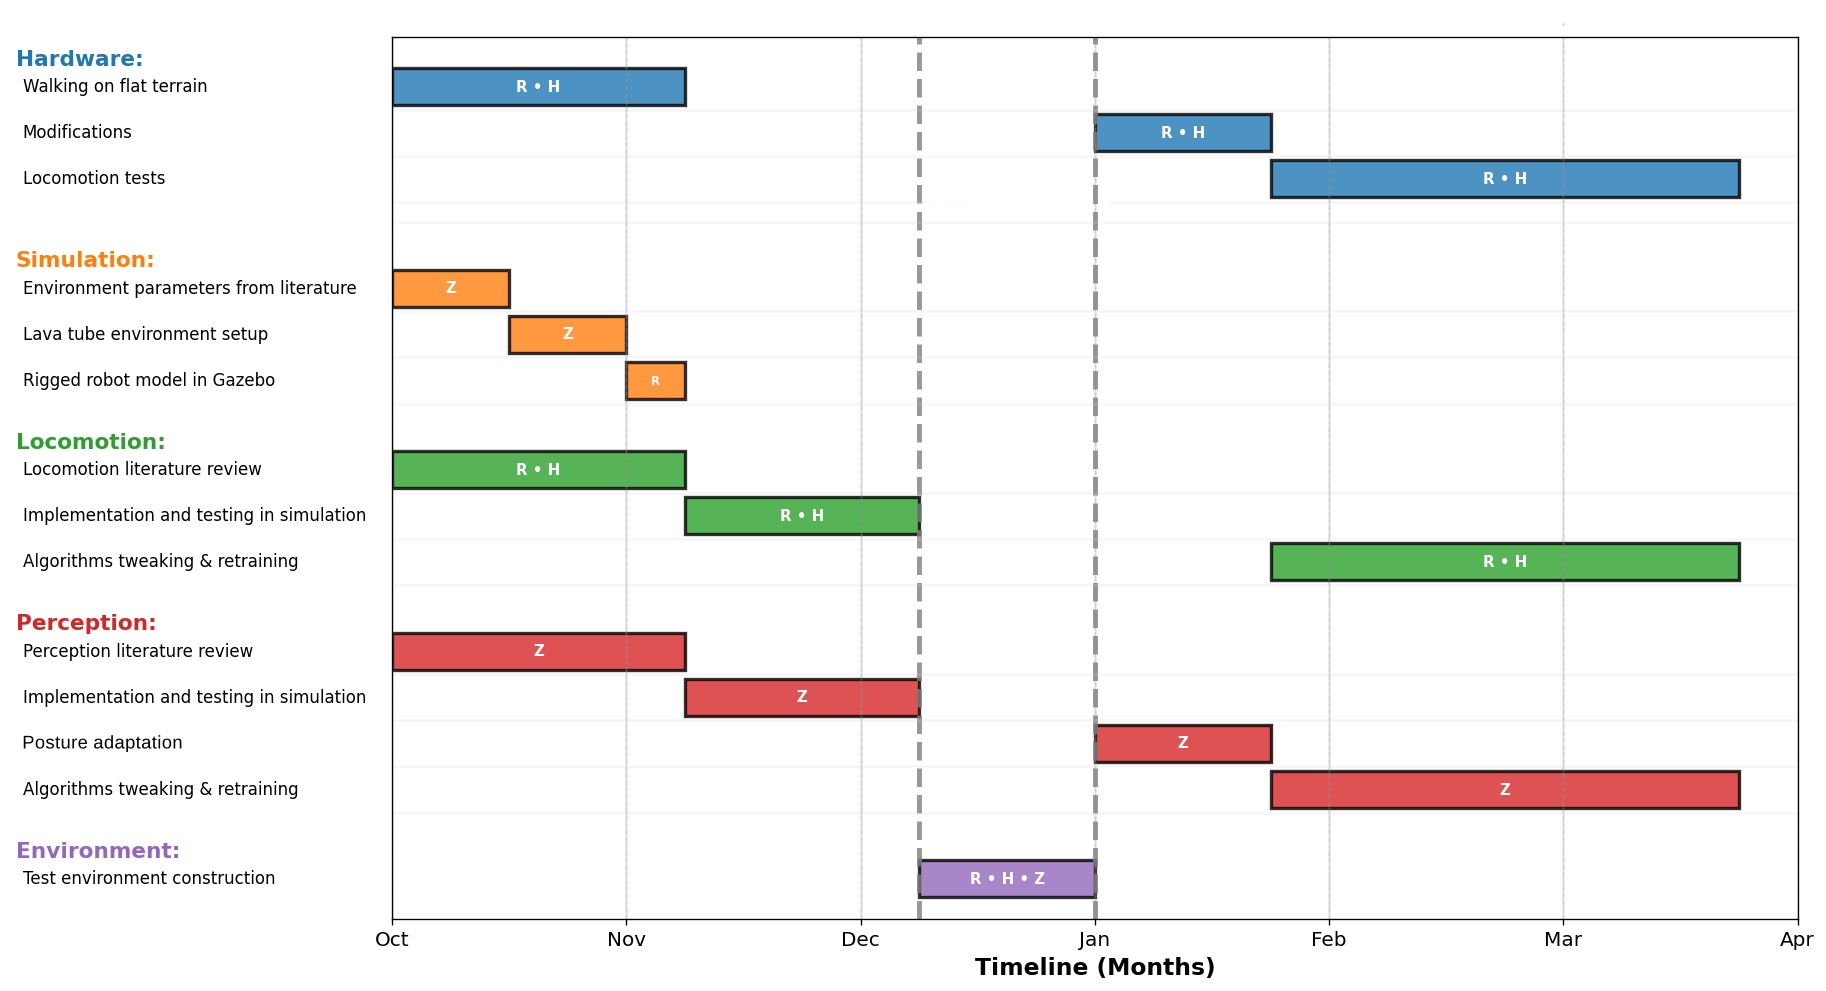
\includegraphics[width=1.0\textwidth]{gantt.png}
    \caption{The Gantt chart for scheduling tasks per team member.}
    \label{fig:gantt}
\end{figure}



\section{Key Challenges}

The project is highly constrained by the hobby-grade hardware. Key challenges include:
\begin{itemize}
    \item \textbf{Actuation Limits:} The motors are really weak as compared to other robots, even ones of the same size, thus making it much harder to put load on the robot or expect it to perform well. This plays a part in simulation as well as we try to accurately model the motor limits.
    \item \textbf{Power Constraints:} Making the robot stand draws 2A of current per side. Each power rail on our SSC-32U servo controller is rated for a maximum of 3A, leaving a critically narrow margin for dynamic movements.
    \item \textbf{Sim-to-Real Gap:} The robot does not have any proprioceptive sensors, so we had to retrofit an IMU and tap the potentiometers for joint state feedback. While these solutions are the most sensible out of everything we could do, this does introduce challenges as the feedback from the sensors is noisy and requires additional work to filter out noise.
    \item \textbf{Novelty of Posture Adaptation:} This is a significantly unexplored topic with approaches most often targetting posture adaptation for flat terrain, so concocting a personal approach deviating from literature is required here. 
\end{itemize}

\chapter{Literature Review}
\label{chap:lit}

\section{Robot Design}

With respect to robot design, there are many factors to consider, such as the robot morphology, type of actuators, sensor suite, and compute capabilities.

Morphology refers to the physical structure of the robot as defined by the number of limbs, joints, and their kinematic alignments. For multi-legged robots, two main morphologies are commonly used: parasagittal and sprawling (see figures \ref{fig:cheetah3} and \ref{fig:thex}). Each of these morphologies can have a varying number of legs, with quadrupeds and hexapods being the most common. Both morphologies have their own advantages and disadvantages. Most prominently, parasagittal robots are more energy efficient, with legs straight below the hip, allowing the robot to stand without exerting torque on the joints. However, they usually have a higher center of mass and a smaller support polygon, making them more susceptible to tipping over during locomotion. On the other hand, sprawling robots, with their legs extending in the lateral direction from the hip, have a much lower center of mass and a wider support polygon, making them more stable, but less energy efficient as the joints must exert torque to hold the body up against gravity even when the robot is standing still.

% \begin{figure}[h!]
%     \begin{minipage}[t]{0.48\textwidth}
%         \centering
%         
\includegraphics[width=\textwidth]{figures/cheetah3.png}
%         \caption{MIT's Cheetah 3, a parasagittal quadruped with 3DoF legs \cite{bledtMITCheetah32018}}
%         \label{fig:cheetah3}
%     \end{minipage}
%     \hfill
%     \begin{minipage}[t]{0.48\textwidth}
%         \centering
%         
\includegraphics[width=\textwidth]{figures/THex.jpeg}
%         \caption{Lynxmotion's T-Hex, a sprawling hexapod with 3DoF legs \cite{THex3DoFHexapod}}
%         \label{fig:thex}
%     \end{minipage}
%     % \caption{Overall caption for both images (optional).}
% \end{figure}

Some examples of state-of-the-art parasagittal robots include the MIT Cheetah 3 \cite{bledtMITCheetah32018}, Boston Dynamics' Spot \cite{Spot}, ETH Zurich's SpaceBok \cite{armSpaceBokDynamicLegged2019}, ANYbotics' ANYmal \cite{hutterANYmalHighlyMobile2016}, IIT's HyQ \cite{seminiHyQDynamicLocomotion}, Unitree B2 \cite{UnitreeB2}, Unitree Go 2 \cite{UnitreeGo2}. All of these robots are quadrupeds having 3 DOF per leg, except for SpaceBok with 2 DOF per leg. On the other hand, examples of sprawling robots include CSIRO's Weaver \cite{bjelonicWeaverHexapodRobot2018}, CTU Prague's HAntR \cite{cizekDesignConstructionRoughTerrain2021}, and Lynxmotion's T-Hex \cite{THex3DoFHexapod}, which have 5-DOF, 4-DOF, and 3-DOF legs respectively. While parasagittal quadrupeds and sprawling hexapods are the most common morphologies, other morphologies such as parasagittal hexapods, for example DOBOT's Hexplorer \cite{DOBOTHEXAPODRobot} and RHex \cite{PDFRHexSimple}, and sprawling quadrupeds, for example the TITAN-XIII \cite{PDFTITANXIIISprawlingtype}, have also been developed.

Beyond morphology, the actuation scheme fundamentally dictates a robot's dynamic capabilities and its ability to negotiate rough terrain. High-performance platforms rely on torque-controlled actuators that allow the robot to act as a virtual spring, absorbing unexpected impacts from uneven ground. For example, the MIT Cheetah 3 \cite{bledtMITCheetah32018} utilizes custom quasi-direct drive (QDD) actuators, which combine high-torque brushless motors with low-ratio gearboxes to achieve high mechanical transparency and backdrivability. ANYmal \cite{hutterANYmalHighlyMobile2016} and StarlETH \cite{hutterSTARLETHCOMPLIANTQUADRUPEDAL2012} employ Series Elastic Actuators (SEAs), placing a physical spring between the motor and the joint to absorb shocks and store energy, while the HyQ platforms \cite{seminiHyQDynamicLocomotion} rely on hydraulic cylinders for extreme force density and impact resistance. Similarly, the industrial-grade Unitree B2 \cite{UnitreeB2} utilizes high-torque-density motors capable of supporting up to 120 kg payloads over severe terrain. To bridge the gap to more accessible hardware, open-source research platforms like PADWQ \cite{kimPADWQDesignControl2021} achieve similar dynamic transparency by leveraging custom low-gear-ratio transmissions and 3D-printed components. Conversely, low-cost and educational platforms, such as the Stanford Pupper \cite{YerbertDingoQuadrupedBase}, HAntR \cite{cizekDesignConstructionRoughTerrain2021}, and our T-Hex kit \cite{THex3DoFHexapod}, utilize position-controlled hobby servos. While affordable and lightweight, these rigid actuators lack force feedback (and often, any kind of feedback) and cannot naturally absorb shocks, requiring specialized algorithms to detect and react to contacts.

To traverse rough terrain and assess spatial constraints, the robot needs a suite of sensors, which is generally divided into proprioceptive and exteroceptive sensors. Proprioceptive sensors measure the robot's internal state; almost all modern legged robots feature high-resolution joint encoders to measure joint positions, torque sensors to measure joint efforts, and a central Inertial Measurement Unit (IMU) placed near the Center of Mass (CoM) to estimate body orientation, position, acceleration, and linear and angular velocity. Contact sensors, detecting when the feet make and break contact with the ground, are also common. Relying heavily on this high-frequency proprioceptive feedback, platforms such as the Ghost Robotics Vision 60 \cite{Vision60Ghost} emphasize blind locomotion to traverse tall grass or deep water where cameras might fail. Similarly, the MIT Cheetah 3 \cite{bledtMITCheetah32018} utilizes proprioception and robust sensor fusion \cite{bledtContactModelFusion2018} to run and gallop at high speeds, bounding up stairs and traversing over unstructured terrain completely blind. Highly specialized robots like SpaceBok \cite{armSpaceBokDynamicLegged2019} also rely heavily on internal state estimation, integrating precise IMUs and leg kinematics to achieve in-flight attitude control in low-gravity environments.

However, exteroceptive sensors, which measure the outside world, are critical for posture adaptation in confined spaces. State-of-the-art robots like Spot \cite{Spot, boumanAutonomousSpotLongRange2020} and ANYmal \cite{gehringANYmalFieldSolving2021} feature an array of stereo depth cameras placed around the perimeter of the chassis to provide 360-degree close-range obstacle detection, often coupled with a 3D LiDAR at the top of the chassis for long-range spatial mapping. Other platforms achieve environmental awareness through more directional sensing. To achieve similar perceptive capabilities on a budget, platforms like the Unitree Go2 \cite{UnitreeGo2} and PADWQ \cite{kimPADWQDesignControl2021} mount a single forward-facing depth camera (such as an Intel RealSense) or a solid-state LiDAR whereas Weaver \cite{bjelonicWeaverHexapodRobot2018} utilizes stereo cameras to perceive the terrain. 

Finally, running advanced locomotion algorithms (the kinds of which we will discuss in the next section) that take in sensor data and output joint commands requires significant onboard compute capabilities, typically arranged in a hierarchical architecture. The low-level control loop, which is mainly responsible for the actual locomotion itself, that is estimating states, calculating joint commands to move and maintain balance, must run at high frequencies (often between 50 Hz and 1000 Hz) and is usually handled by a dedicated real-time microcomputer. The MIT Cheetah 3 \cite{bledtMITCheetah32018} runs its purely proprioceptive locomotion controller at 1000Hz using a dedicated onboard x86 PC running a real-time operating system. For systems with perception modules, high-level planning tasks, such as processing dense point clouds to localize the robot, assess spatial constraints, build a map, or plan a trajectory run at much lower frequencies (5 Hz to 50 Hz), mainly due to computational expenses, but also due to assumptions regarding how fast the perception data realistically changes. ANYmal \cite{hutterANYmalHighlyMobile2016} employs multiple onboard Intel Core i7 processors, dedicating one exclusively to real-time locomotion control and another entirely to perceptive navigation and mapping \cite{hoellerANYmalParkourLearning2023}. PADWQ \cite{kimPADWQDesignControl2021} explicitly incorporates an onboard GPU to handle its perceptive locomotion.

Considering its sprawling morphology, position-controlled servos with less than 1 Nm peak torque, no integrated feedback, and a low-speed servo controller, the T-Hex, especially with two legs removed, is greatly limited by its hardware as compared to other robots in the similar weight class, requiring us to augment it with the bare-minimum sensors for robust locomotion, and work around the limitations of its actuators and servo controller. Algorithms that require minimal state feedback, such as joint state and body orientation, and can run at low frequencies are most suitable for the T-Hex. This motivates an extensive literature review of locomotion approaches to find the most suitable ones for our hardware.

\section{Locomotion and Perception}

The locomotion of legged robots in various challenging scenarios has been an active area of research for the past few decades. Locomotion controllers for legged robots can be divided into two-main categories: model-free controllers and model-based controllers. Here, the model being referred to is the dynamics model of the robot, which is typically used to relate the forces and torques on the robot's legs to the motion of the robot body\cite{bledtMITCheetah32018, dicarloDynamicLocomotionMIT2018}. 

One of the simplest model-free control techniques to make a legged robot walk is to use an open-loop\footnote{As opposed to closed-loop, which means to incorporate state feedback.} kinematic gait that has each leg follow a pre-computed foot trajectory\cite{sunHexapodRobotKinematics2017}. A controller like this is easy to implement thanks to well-established approaches for deriving legs' kinematic equations, but is expected to perform poorly in anything but flat terrain. A legged robot is a highly dynamic system, and such a controller ignores the dynamics entirely. Furthermore, not incorporating feedback means the controller is blind to when a leg doesn't reach the desired position. If the leg hits an obstacle in the middle of its swing phase blocking its movement, the leg will continue to push against the obstacle, instead of adjusting its trajectory, like by increasing the amplitude of the swing, to overcome it. These factors, combined with the reliance on good gait parameters such as swing amplitude, stride length, and the lateral distance from the hip\footnote{This is only applicable for robots with a sprawling morphology, like T-Hex. For parasagittal robots, such as Spot or ANYmal, the lateral distance from the hip can be 0.}, makes such a controller unsuitable for unstructured terrain. 

Central Pattern Generators (CPGs), inspired by biological neural networks in animal nervous systems, are used in more sophisticated model-free controllers to generate kinematic references for the robot's joints to follow. The implementation of CPGs varies across literature \cite{owakiQuadrupedRobotExhibiting2017, barasuolReactiveControllerFramework2013, fukuokaSimpleRuleQuadrupedal2015, AdaptiveDynamicWalking, chenLocomotionControlSensordriven2016, parkStableModifiableWalking2013, zhangTrotGaitDesign2014}, but at a high-level, a CPG is attached to each joint in the robot and generates oscillatory signals that act as reference joint trajectories. CPGs in each joint can communicate with each other implicitly through mathematical coupling, which allows for designing specific gaits that rely on phase differences between groups of legs. Performance of CPGs also relies on the choice of parameters, and learning-based methods or derivative-free optimization techniques like evolutionary algorithms are often used to find the best set of parameters by simulating the robot in virtual terrain \cite{liParameterTuningCPGs2015, renMultipleChaoticCentral2015, endoLearningCPGbasedBiped2008}. When state feedback is incorporated into such controllers, they can be surprisingly robust even in non-flat terrain involving slopes, stairs, and unstructured elements such as pebbles and stones \cite{AdaptiveDynamicWalking, barasuolReactiveControllerFramework2013, chenLocomotionControlSensordriven2016}.

Recently, Deep Reinforcement Learning (DRL) has been under the spotlight for learning robust locomotion controllers for legged robots. Proximal Policy Optimization (PPO), a policy-gradient method developed at OpenAI \cite{schulmanProximalPolicyOptimization2017}, is used when training DRL-based controllers due to its impressive performance particularly for tasks related to robot locomotion and manipulation. In PPO, two separate neural networks are trained simultaneously. The value network is responsible for learning how good each state is, whereas the policy network learns the best actions to take at each state - only the latter is actually used after training. To train the two networks, many instances of robots are simulated in virtual environments \cite{rudinLearningWalkMinutes2022}. NVIDIA's Isaac Lab \cite{nvidiaIsaacLabGPUAccelerated2025} provides pre-developed plug-and-play packages for training the locomotion of any legged robot in a variety of environments. To minimize the sim-to-real gap, domain randomization is used to simulate unmodeled factors and wear and tear of hardware, which makes the controller robust to external disturbances. DRL-based locomotion controllers are successful in a wide variety of terrains and demonstrate impressive dynamic movement abilities \cite{tahaDevelopingHexapodLocomotion2025, mikiLearningRobustPerceptive2022, leeLearningQuadrupedalLocomotion2020, choiLearningQuadrupedalLocomotion2023, margolisRapidLocomotionReinforcement2022, tanSimtoRealLearningAgile2018, rudinCatlikeJumpingLanding2022, rudinAdvancedSkillsLearning2022, nahrendraDreamWaQLearningRobust2023, kimDeepReinforcementLearning2026}.

Model-based approaches require some dynamic model of the robot. A perfectly accurate dynamic model is usually too complex to be directly used; however, under specific assumptions, a simplified dynamic model can be used to approximate the robot's dynamics. 

Among the first model-based approaches to legged locomotion used the Simple Linear Inverted Pendulum (SLIP) model, first proposed by Cavagna \cite{cavagnaMechanicalWorkTerrestrial1977} for modeling locomotion of animals. The SLIP model can be visualized as a point mass on a spring that is passive and conservative, representing the body and leg respectively. With slight modifications, the SLIP model has been used to design impressive locomotion controllers robust to disturbances \cite{raibertTrottingPacingBounding1990, RunningFourLegs, poulakakisStabilityPassiveDynamics2006}. However, the SLIP model isn't directly applicable to all morphologies of robots, including sprawling legged robots such as T-Hex. Furthermore, such approaches usually rely on instantaneous analytical solutions which requires making stric t assumptions regarding the motion of the robot, such as assuming a contact schedule for legs, which can be violated in unstructured terrain.

Modern approaches move away from analytical solutions to optimization-based controllers and use more complex and accurate dynamic models \cite{bledtMITCheetah32018, dicarloDynamicLocomotionMIT2018, kolvenbachTraversingSteepGranular2021, huConstrainedModelPredictive2019, oshinDifferentiableRobustModel2024, grandiaDesignControlBipedal2024, parkOnlinePlanningAutonomous2015, bledtPolicyRegularizedModel, dingRealtimeModelPredictive2019, nosratiRegularizedModelPredictive2025, wieberTrajectoryFreeLinear2006, herdtWalkingThinkingIt2010, prattVirtualModelControl1995, hutterSTARLETHCOMPLIANTQUADRUPEDAL2012, xieIntuitiveApproachQuadruped2015, kocoHybridComplianceControl2019, liuResearchPostureControl2020, torresVirtualModelControl, chenVirtualModelControl2020}. Such controllers plan a center of mass trajectory, typically based on user commands of linear and angular velocity of the body, and then optimize for ground reaction forces exerted by the stance legs to enforce the desired dynamics on the robot's center of mass, such as zero roll and pitch velocity to remain upright or zero vertical acceleration to maintain a base height. Swing legs are typically commanded to follow a reference swing trajectory as is typical with other types of locomotion controllers. 

However, the robot also has to consider how to adjust itself in order to minimize collisions with the walls and ceiling in confined environments. For that, it requires a way of sensing the environment that mere proprioceptive sensors cannot provide. Exteroceptive sensors, such as RGB-D cameras and LiDARs, that provide point clouds containing depth information of the surrounding terrain prove to be a necessity. To understand the environment's geometry, one proposed method is to split the pointcloud into patches and fit local planes using covariance eigenanalysis, yielding slope and roughness \cite{3DSLAMUsing}. This can be expanded upon to include per-cell uncertainty and height leading to a probabilistic elevation map \cite{fankhauserRobotcentricElevationMapping2014, PDFProbabilisticTerrain}. However, these elevation maps do not consider ceilings or overhangs, which introduce multiple z-values. To solve this, the OctoMap \cite{hornungOctoMapEfficientProbabilistic2013} provides full 3D occupancy for the entire space instead of estimating surfaces. On the other hand, Voxblox \cite{oleynikovaVoxbloxIncremental3D2017} utilizes signed distance fields (SDFs) to allow clearance or available space to be obtained efficiently. From there, traversibility; that is, a metric determining safer spots for the robot to go to; is computed. This could range from determining rules for desired slope, roughness, and clearance to learning foothold quality via a network and robot experience. Now, given traversability, the robot must choose how to adapt its configuration or posture to fit in; this can be achieved via abstracting the robot into a deformable bounding box and creating a trajectory of desired body postures \cite{buchananWalkingPostureAdaptation2019, buchananPerceptiveWholebodyPlanning2021}. Perception-based locomotion has also seen significant integration in RL as demonstrated by Miki et al. who used elevation maps as inputs into RL policy \cite{mikiLearningRobustPerceptive2022}. These were replaced with full 3D volumetric representation for confined spaces \cite{mikiLearningWalkConfined2024}. 


\chapter{Software Requirement Specification (SRS)}
\label{chap:srs}

% --- 1. Introduction ---
The project is divided into three core streams:
\begin{itemize}
    \item \textbf{Locomotion:} Developing capability of the robot to traverse rough terrain
    \item \textbf{Perception:} Developing capability of the robot to sense its environment and take decisions, e.g. with regards to posture adaptation
    \item \textbf{Simulation:} Developing an accurate virtual environment to safely implement, test, and iterate over the locomotion and perception strategies before hardware deployment
\end{itemize}

% --- 2. Functional Requirements ---
\section{Functional Requirements}

\subsection{Simulation}
\begin{itemize}
    \item The simulation system must allow for randomly generating environments
    \item The simulated environments must have rough terrain
    \item The simulated environments must have narrow passages, areas with low ceilings, and protrusions from the ground to test posture adaptation
    \item The generation process must include parameters for adjusting roughness in terrain, ground friction, range of width and height of passages, and range of size of protrusions
    \item The simulation system must support physics
    \item The T-Hex robot must be simulated with user-defined mass properties
\end{itemize}

\subsection{Perception}
\begin{itemize}
    \item The robot must be integrated with a camera to be attached on the robot in simulation
    \item The robot must be able to build a map of the immediate environment in simulation, i.e., what is directly ahead of the robot 
    \item The robot must be able to use a map of the immediate environment in simulation to make decisions to switch to a narrower posture to pass through thin passages, a shorter posture to pass under low ceilings, or a posture with higher body clearance to pass over protrusions
\end{itemize}

\subsection{Locomotion}
\begin{itemize}
    \item The robot, in both simulation and hardware, should be able to walk on flat and rough terrain
    \item The robot, in both simulation and hardware, should be able to adapt its posture in both flat and rough terrains
    \item The robot, in both simulation and hardware, must be teleoperable - it should take a target position relative to itself as input and execute a straight line trajectory to reach it, adjusting to the terrain and obstacles
\end{itemize}
% \begin{itemize}
%     \item \textbf{Gait Scheduling:}
%         \item The system must implement an open-loop kinematic gait for basic walking and testing.
%         \item The system must implement a dynamic gait scheduler that determines which legs are in the stance phase and which are in the swing phase at any given time.
%     \item \textbf{Trajectory Generation:}
%         \item The system must compute a desired Center of Mass (CoM) trajectory based on operator commands and the current gait schedule.
%         \item The system must generate smooth swing leg trajectories (e.g., using splines) to move a leg from its current position to a desired foothold.
%     \item \textbf{Dynamic Control:}
%         \item The system must plan optimal footholds for swing legs based on the robot's velocity and terrain data (e.g., using Raibert's heuristic).
%         \item The system must calculate the optimal Ground Reaction Forces (GRFs) for all stance legs to maintain balance and follow the desired CoM trajectory. This shall be achieved via a model-based controller (e.g., Balance Controller with QP or Convex MPC).
%         \item The system must translate desired forces (for stance legs) and desired positions (for swing legs) into final joint torque commands using a Joint PD Controller.
%     \item \textbf{Posture Adaptation:}
%         \item The system must use perception data to autonomously adapt the robot's body posture (height, roll, pitch).
%         \item The system must be able to lower its posture to navigate under low overhangs and narrow its posture to pass through thin gaps.
    
%     \item The system must estimate the robot's Center of Mass (CoM) state; that is, its position, velocity, and orientation.
%     \item The system must be able to detect whether a leg is in contact with the ground (stance) or in the air (swing).
% \end{itemize}

% --- 3. Non-Functional Requirements ---
\section{Non-Functional Requirements}

\begin{itemize}
    \item The robot should be able to walk in terrains with local vertical step size up to 8cm
    \item The robot should be able to walk in terrains with local slope up to 15 degrees
    \item The robot should be able to pass through passages as narrow as 38cm in simulation
    \item The robot should be able to pass through areas with ceilings as low as 16cm in simulation
    \item The robot should be able to pass over protrusions of up to 6cm in simulation
    \item The robot should be able to walk in terrains with friction coefficient of 0.5-0.7
    \item The robot should be able to walk in terrains with sand, ash, and pebbles as big as 1cm
    \item There must be at least three ``postures'' that the robot should be able to move in: a shorter posture, a regular posture, and a posture with higher body clearance in simulation
    \item For data integrity purposes, there must be a Docker image containing everything necessary to run the simulation of the robot in randomly generated environments
    \item The entire codebase must be well-commented with citations included in either the README or as comments in the file themselves for code that is taken or adopted from someplace else
    \item The entire codebase must be well-structured and maintained with complete version control on GitHub to allow for backups in case of catastrophe
    \item Documents detailing the robot's hardware architecture and its locomotion and perception strategy must be prepared
\end{itemize}

% \subsection{Performance}
% \begin{itemize}
%     \item The system must generate the multi-elevation map and pass it to the path planner at a frequency of 1-4 Hz.

%     \item The mapping algorithms must be fast enough to avoid bottlenecks in the perception pipeline.

%     \item The height information must be granular enough for the robot to navigate terrain and obstacles.

%     \item The system must cluster sensor data into "floor" and "ceiling" elevations with sufficient accuracy.

%     \item The perception system must account for drift in odometry.

%     \item The system map must maintain reliability of data and discard outdated information over time.

%     \item The system must account for sensor bias, variance, and noise/

%     \item The system must be able to function in a real environment imitating a lava tube.

%     \item The dynamic balance controller must execute in real-time to ensure stability. The low-level Joint PD Control loop must run at a frequency of at least 500 Hz.
%     \item The robot must draw a stable current to operate. The system must manage power, noting that standing alone draws 4A. The final design should explore battery operation.
% \end{itemize}

% % \subsection{Security}
% % \begin{itemize}
% %     \item \textbf{Control Link:} Any wireless communication between the operator GUI and the robot must be encrypted to prevent unauthorized commands.
% %     \item \textbf{Onboard System:} The Raspberry Pi or other onboard computer must be hardened (e.g., disabled default passwords, firewall) to prevent unauthorized network access.
% % \end{itemize}

% \subsection{Reliability}
% \begin{itemize}
%     \item The system must be robust against general hardware failures. 
%     \item The control software must, given significant unexpected contact or sensor failures, enter a safe state immediately without further damage.
%     \item The RPi or SSC32 should not crash unexpectedly.
% \end{itemize}

% \subsection{Usability}
% \begin{itemize}
%     \item The simulation GUI must be easy enough for a typical robotics undergraduate to control the robot.
%     \item The simulation environment and its parameters must be easy to configure.
% \end{itemize}

% \subsection{Data Integrity}
% \begin{itemize}
%     \item Sensor data must be timestamped accurately to ensure proper state estimation.
%     \item The state estimator must validate inputs from the sensor to minimize robot state error.
% \end{itemize}

% \subsection{Backup}
% \begin{itemize}
%     \item A remote repository must be set up for version control of all code.
%     \item Logs must be kept for metrics obtained from simulation and physical trials.
% \end{itemize}

\section{Use Cases}
We have only one user: the Operator. For that, the following use cases are defined:
\begin{itemize}
    \item \textbf{Commands:} The operator gives position commands relative to the robot
    \item \textbf{Adjust simulation parameters:} The operator is able to adjust the parameters of the simulation environment
    \item \textbf{Generate simulation environment:} The operator is able to generate simulation environments
    \item \textbf{Pick and place simulated robot:} The operator is able to move the simulated robot by picking it up and placing it at the desired position
\end{itemize}

\begin{figure}[H]
    \centering
    % --- NOTE: You must create this image file (use_case_diagram.png) ---
    % --- You can use a tool like Lucidchart or diagrams.net      ---
    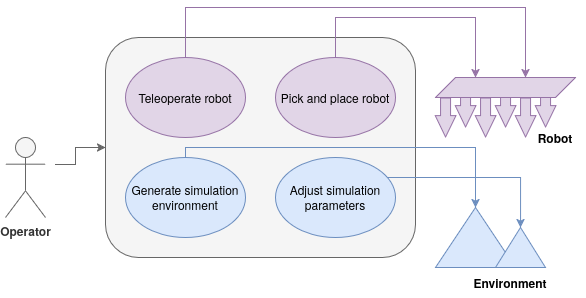
\includegraphics[width=0.6\textwidth]{UseCase.png}
    \caption{Use Case Diagram for the Legged Robot System.}
    \label{fig:use_case}
\end{figure}

\section{Block Diagrams}



\subsection{Perception}


In simulation, the camera takes in the environment and processes it as RGB-D data. It also possesses the IMU data which will tell about the robot's state. Both of these are used to create an elevation map for the robot to not only know where it is in space, but also how to navigate its environment as well as obstacles. There are converted to a signed distance field; that is, a field determining where is safe for the robot to proceed without collision; which lead to vertical and lateral clearance that serve as the basis for posture adaptation. This outputs a posture adaptation signal determining a desired height for the robot, which is sent to the locomotion algorithm. (The width is inferred from the height as described later.)


\begin{figure}[H]
    \centering
    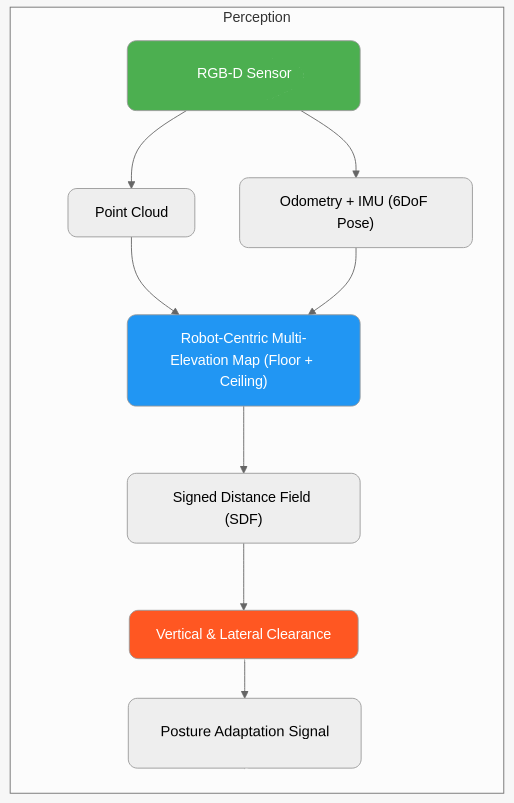
\includegraphics[width=0.5\linewidth]{Perception Diagram.png}
    \caption{Perception Diagram for the Legged Robot System.}
    \label{fig:perception}
\end{figure}

\subsection{Locomotion}

The first of the three locomotion algorithms we have covered is the simplest: the kinematic gait. This operates on a gait schedule, which defines stance and swing legs with their own trajectories. Once generated, the trajectories are tracked before sent as motor commands.

\begin{figure}[H]
    \centering
    % --- NOTE: You must create this image file (use_case_diagram.png) ---
    % --- You can use a tool like Lucidchart or diagrams.net      ---
    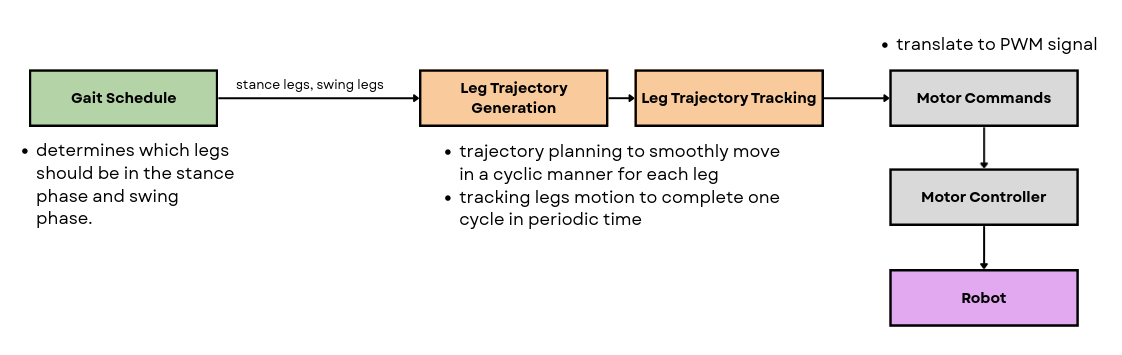
\includegraphics[width=1.0\textwidth]{Locomotion0.png}
    \caption{Kinematic Locomotion Diagram for the Legged Robot System.}
    \label{fig:kinematic_locomotion}
\end{figure}


The next diagram represents the general locomotion architecture that is observed in literature. Based on user commands and the persistent gait schedule, a trajectory for the robot's center of mass is planned, which is used to solve for the forces exerted by the legs in stance (i.e., in contact with the ground) and to generate the trajectories to be generated by the legs in swing. These forces and desired positions are converted into motor commands that are sent to some motor controller and then to the motors. The robot's states (joint positions, roll, pitch, yaw) are incorporated at different steps to ensure robustness.


\begin{figure}[h!]
    \centering
    % --- NOTE: You must create this image file (use_case_diagram.png) ---
    % --- You can use a tool like Lucidchart or diagrams.net      ---
    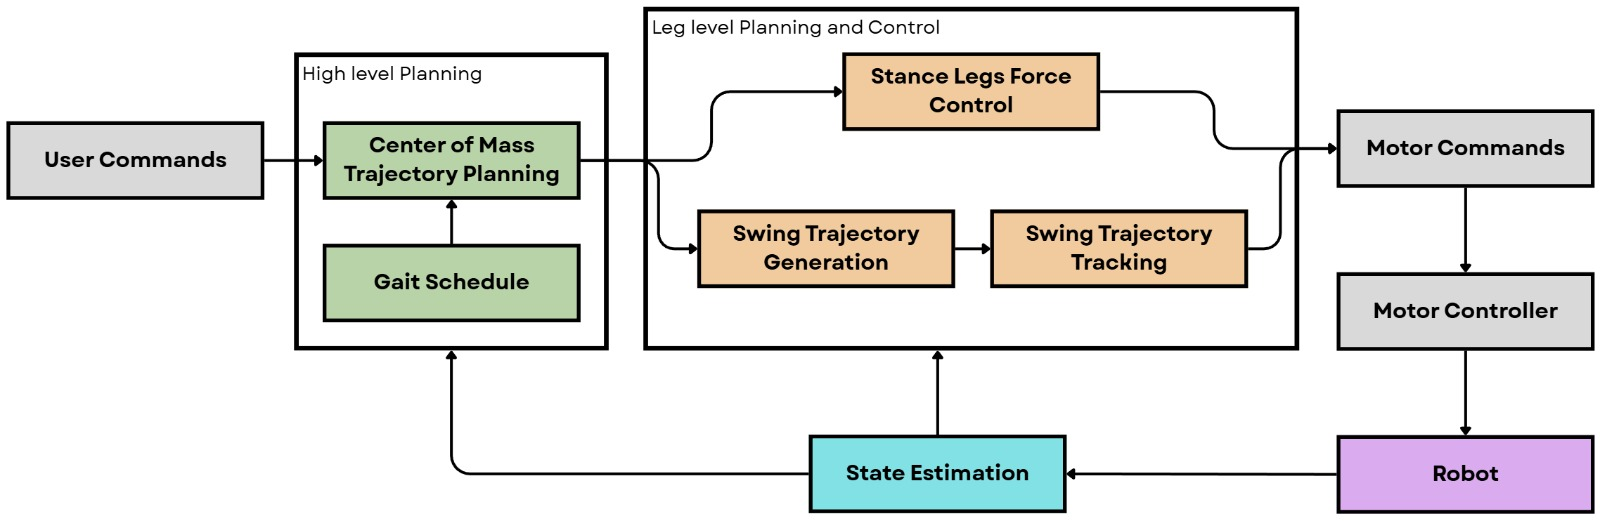
\includegraphics[width=1.0\textwidth]{Locomotion Diagram.png}
    \caption{Dynamic Locomotion Diagram for the Legged Robot System.}
    \label{fig:dynamic_locomotion}
\end{figure}

A third and significant locomotion architecture is that of reinforcement learning (RL). In this case, the policy network starts with user commands and passes its predicted movements as motor commands. Similarly to control, the state estimation segment sends feedback to the network, which adjusts itself accordingly and repeats the cycle. In our case, this particular paradigm's flavor is mixed with a deep learning network, thus being deep reinforcement learning (DRL).

\begin{figure}[h!]
    \centering
    % --- NOTE: You must create this image file (use_case_diagram.png) ---
    % --- You can use a tool like Lucidchart or diagrams.net      ---
    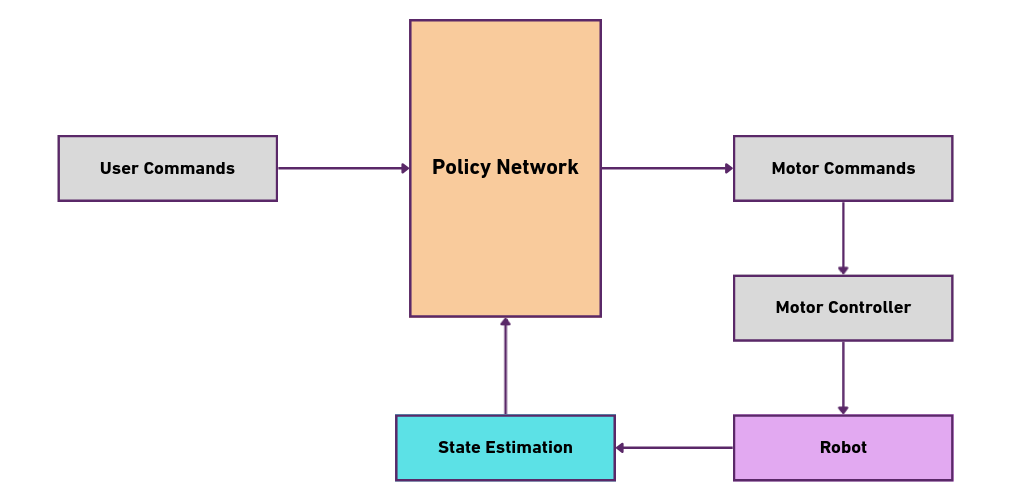
\includegraphics[width=1.0\textwidth]{Locomotion2.png}
    \caption{DRL Locomotion Diagram for the Legged Robot System.}
    \label{fig:drl_locomotion}
\end{figure}


\subsection{Hardware}

\begin{figure}[h!]
    \centering
    % --- NOTE: You must create this image file (use_case_diagram.png) ---
    % --- You can use a tool like Lucidchart or diagrams.net      ---
    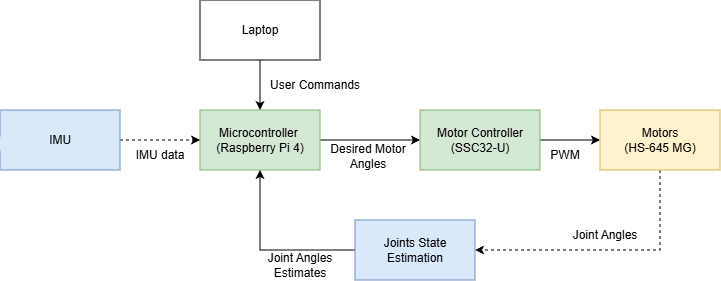
\includegraphics[width=1.0\textwidth]{Hardware Diagram.png}
    \caption{Hardware Diagram for the Legged Robot System. Lines indicate the flow of data, with dotted lines indicating the robot states or world states being observed}
    \label{fig:hardware}
\end{figure}

Our system contains hardware modules depicted in the diagram above. The microcontroller receives user commands from the user's laptop, IMU data from the IMU, and estimates of the robot legs' joint angles from some state estimation method (e.g., motor encoders or motion capture cameras). The microcontroller runs the locomotion algorithms and outputs desired motor angles to the separate motor controller. The motor controller then generates pulse width modulation (PWM) signals that are received by the motors.


\chapter{Software Design Specification (SDS)}
\label{chap:sds}

\section{Software Design}

With regards to our project, we shall consider our simulation as software for the SDS. Hence, this subsection explains the overall design of the simulation system including a UML class diagram.

This particular system is structured around three core modules: \textbf{Environment}, \textbf{Perception}, and \textbf{Locomotion}. These modules interact to allow for teleoperating the robot with posture adaptation on rough terrain. 

Figure \ref{fig:uml_class_diagram} shows the UML class diagram.

\begin{figure}[h!]
    \centering
    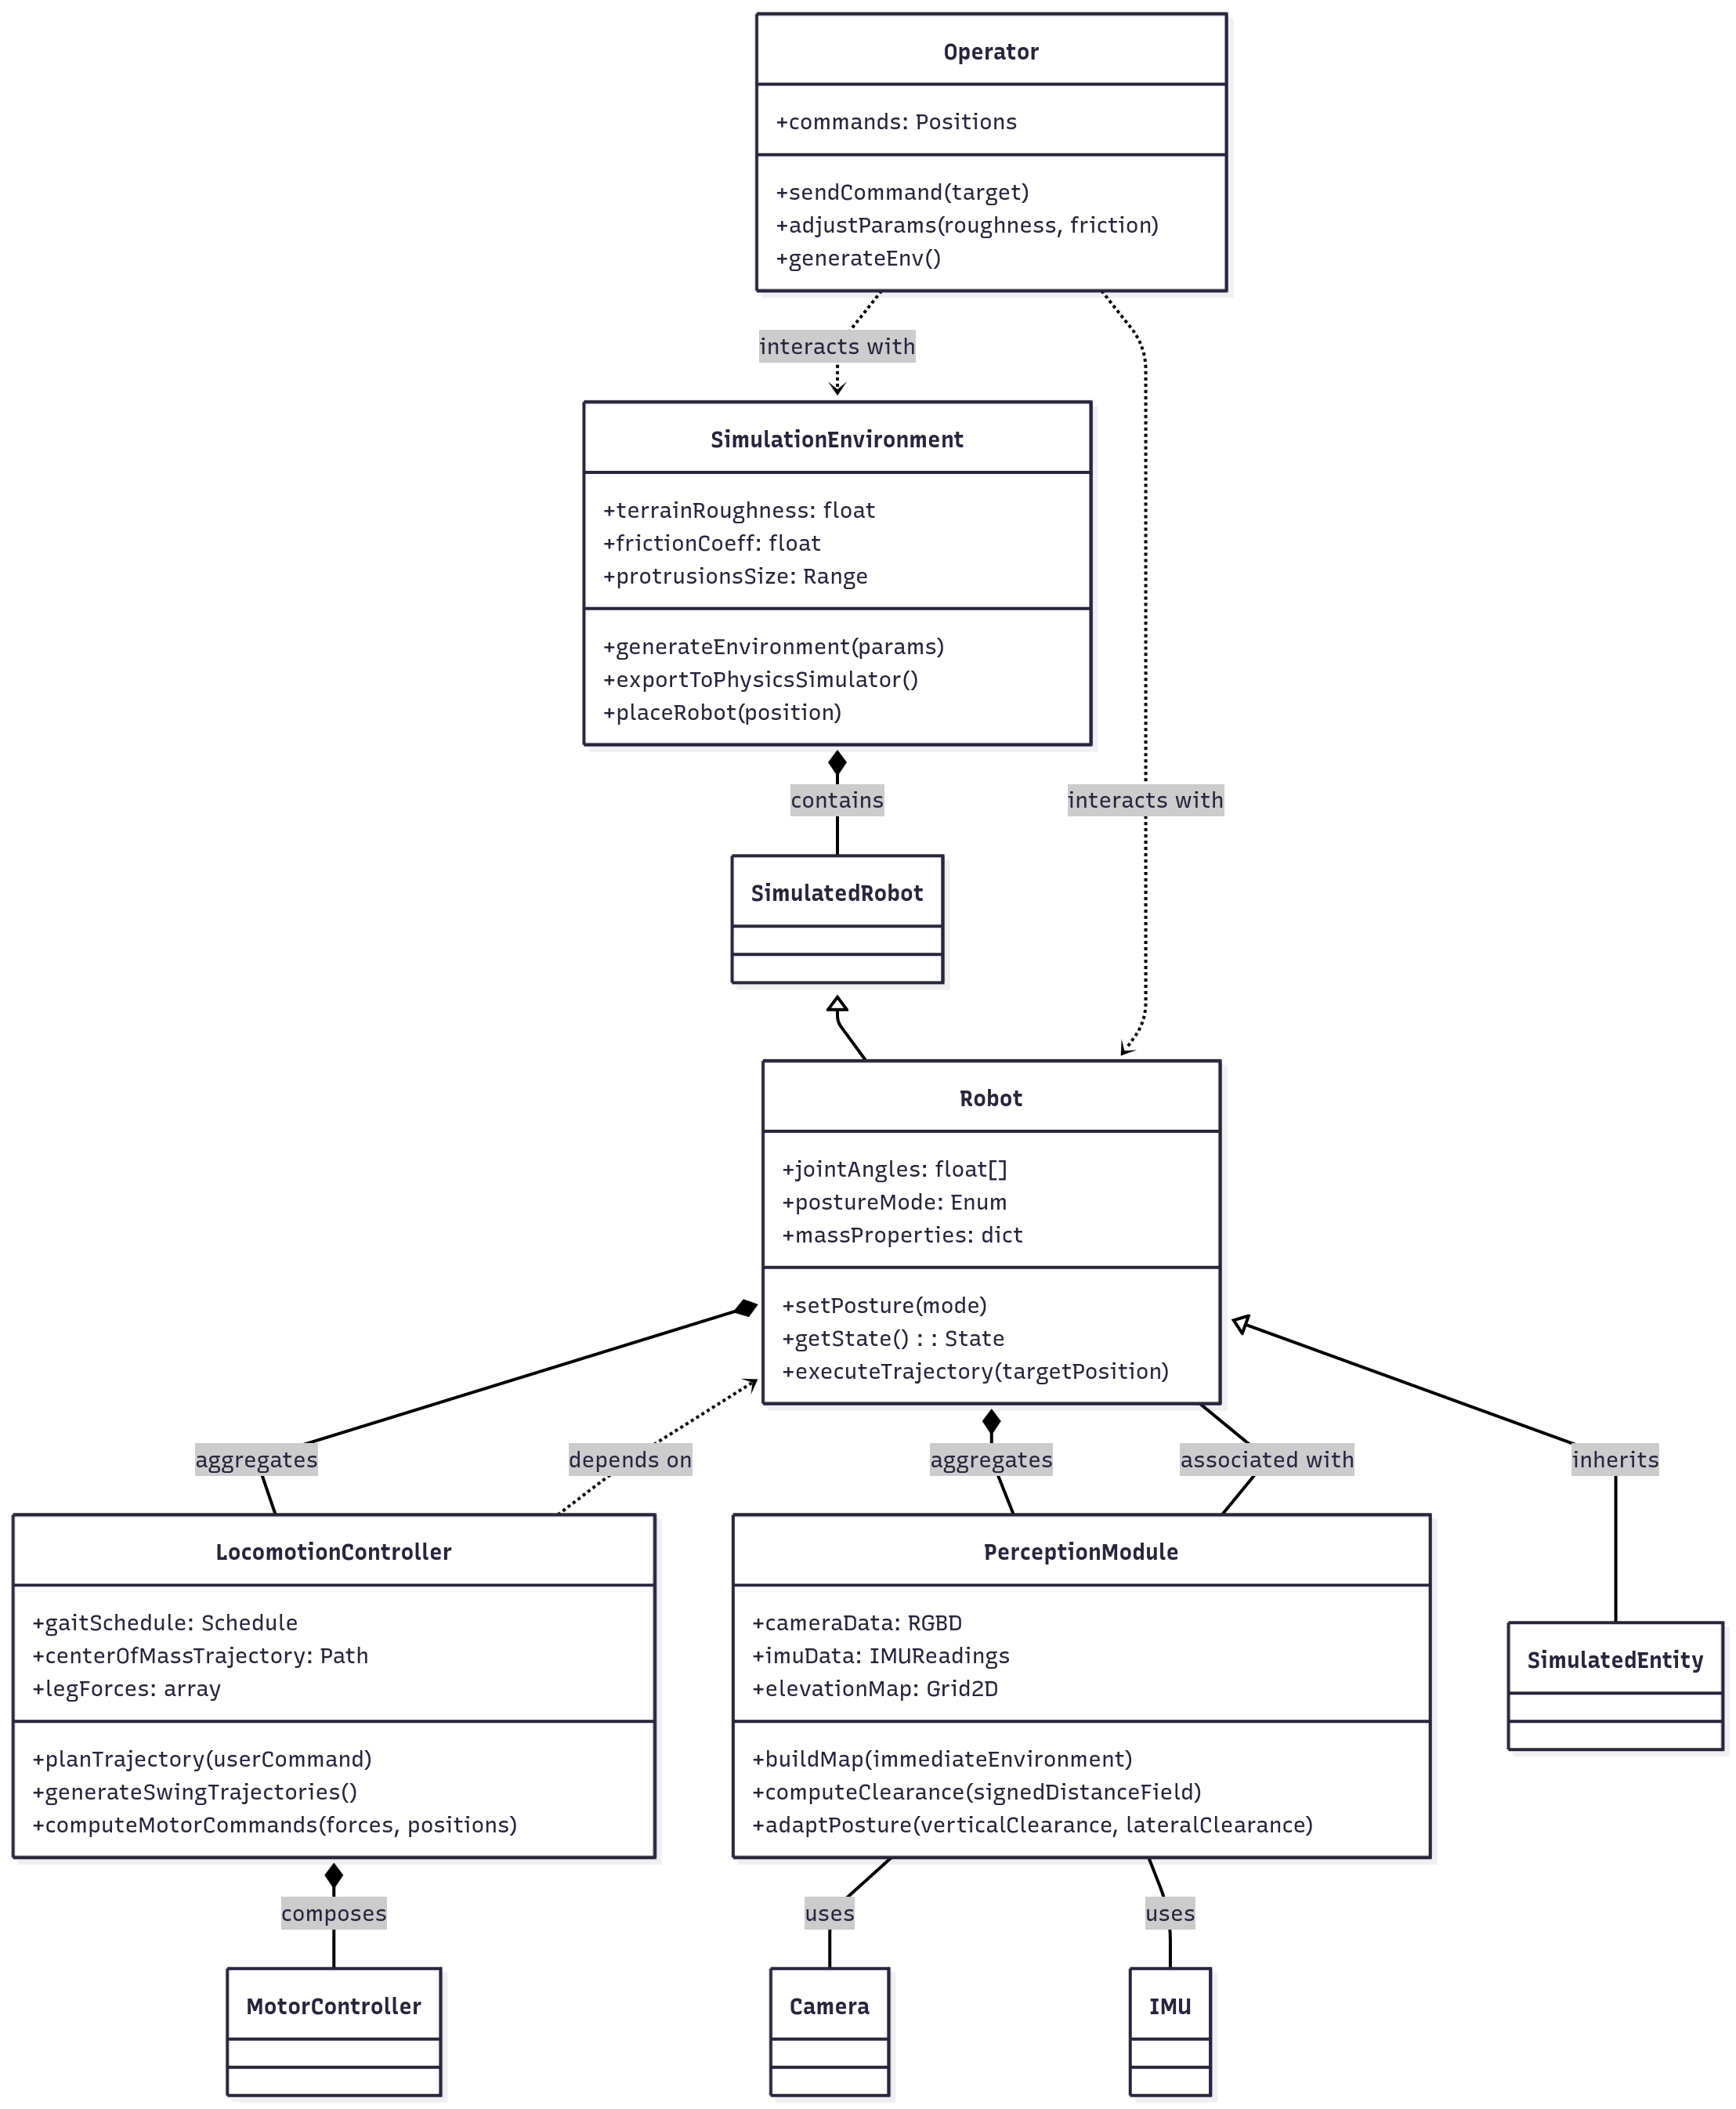
\includegraphics[width=0.85\textwidth]{full.png}
    \caption{Class Diagram for the Legged Robot System.}
    \label{fig:uml_class_diagram}
\end{figure}

The Operator acts as the user interface where the user teleoperates the robot. They also have the liberty to adjust the parameters of the environment such as terrain roughness and friction. The SimulationEnvironment is where the testing happens. It is reliant on the mentioned parameters and generates the environment to show to the physics simulator (Gazebo). Then, the SimulatedRobot is placed within the scene. The Robot is the T-Hex in simulation and manages state information while executing commanded trajectories. It aggregates both the LocomotionController and PerceptionModule; the former manages gaits and trajectories through Ground Reaction Forces for legs in stance and smooth swing leg trajectories to send to the MotorController which executes the commands, and the latter is where the robot senses data from the environment via RGB-D andIMU readings to construct the elevation map. This map is used to calculate clearance; that is, collision-free space; through a signed distance field. This is used to adapt the robot's posture based on the vertical and lateral clearance.

\section{Data Design}

While we do not need persistent data and hence a database, it is worth discussing data structures used in the project. All data is managed within simulation and Docker environment. This data flows through Figures \ref{fig:locomotion_diagram} and \ref{fig:perception_diagram}, and the hardware data path in a physical build is shown in Figure \ref{fig:hardware_diagram}.

The most important data structure is the Elevation Map. It is a 2D grid entity timestamped for accuracy meant to store terrain heights. From here is derived the Signed Distance Field (SDF) which models clearance by retrieving distance values to obstacles. 

The robot's behavioral data relies on Posture Parameters, a structure defining modes using attributes
namely leg spread, fixed body height, etc. On the other hand, the environment relies on Simulation Parameter which are roughness, friction range, maximum protrusion size (6cm), etc. For brevity's sake, we shall not be including the kinematic and DRL diagrams here.

\begin{figure}[h!]
    \centering
    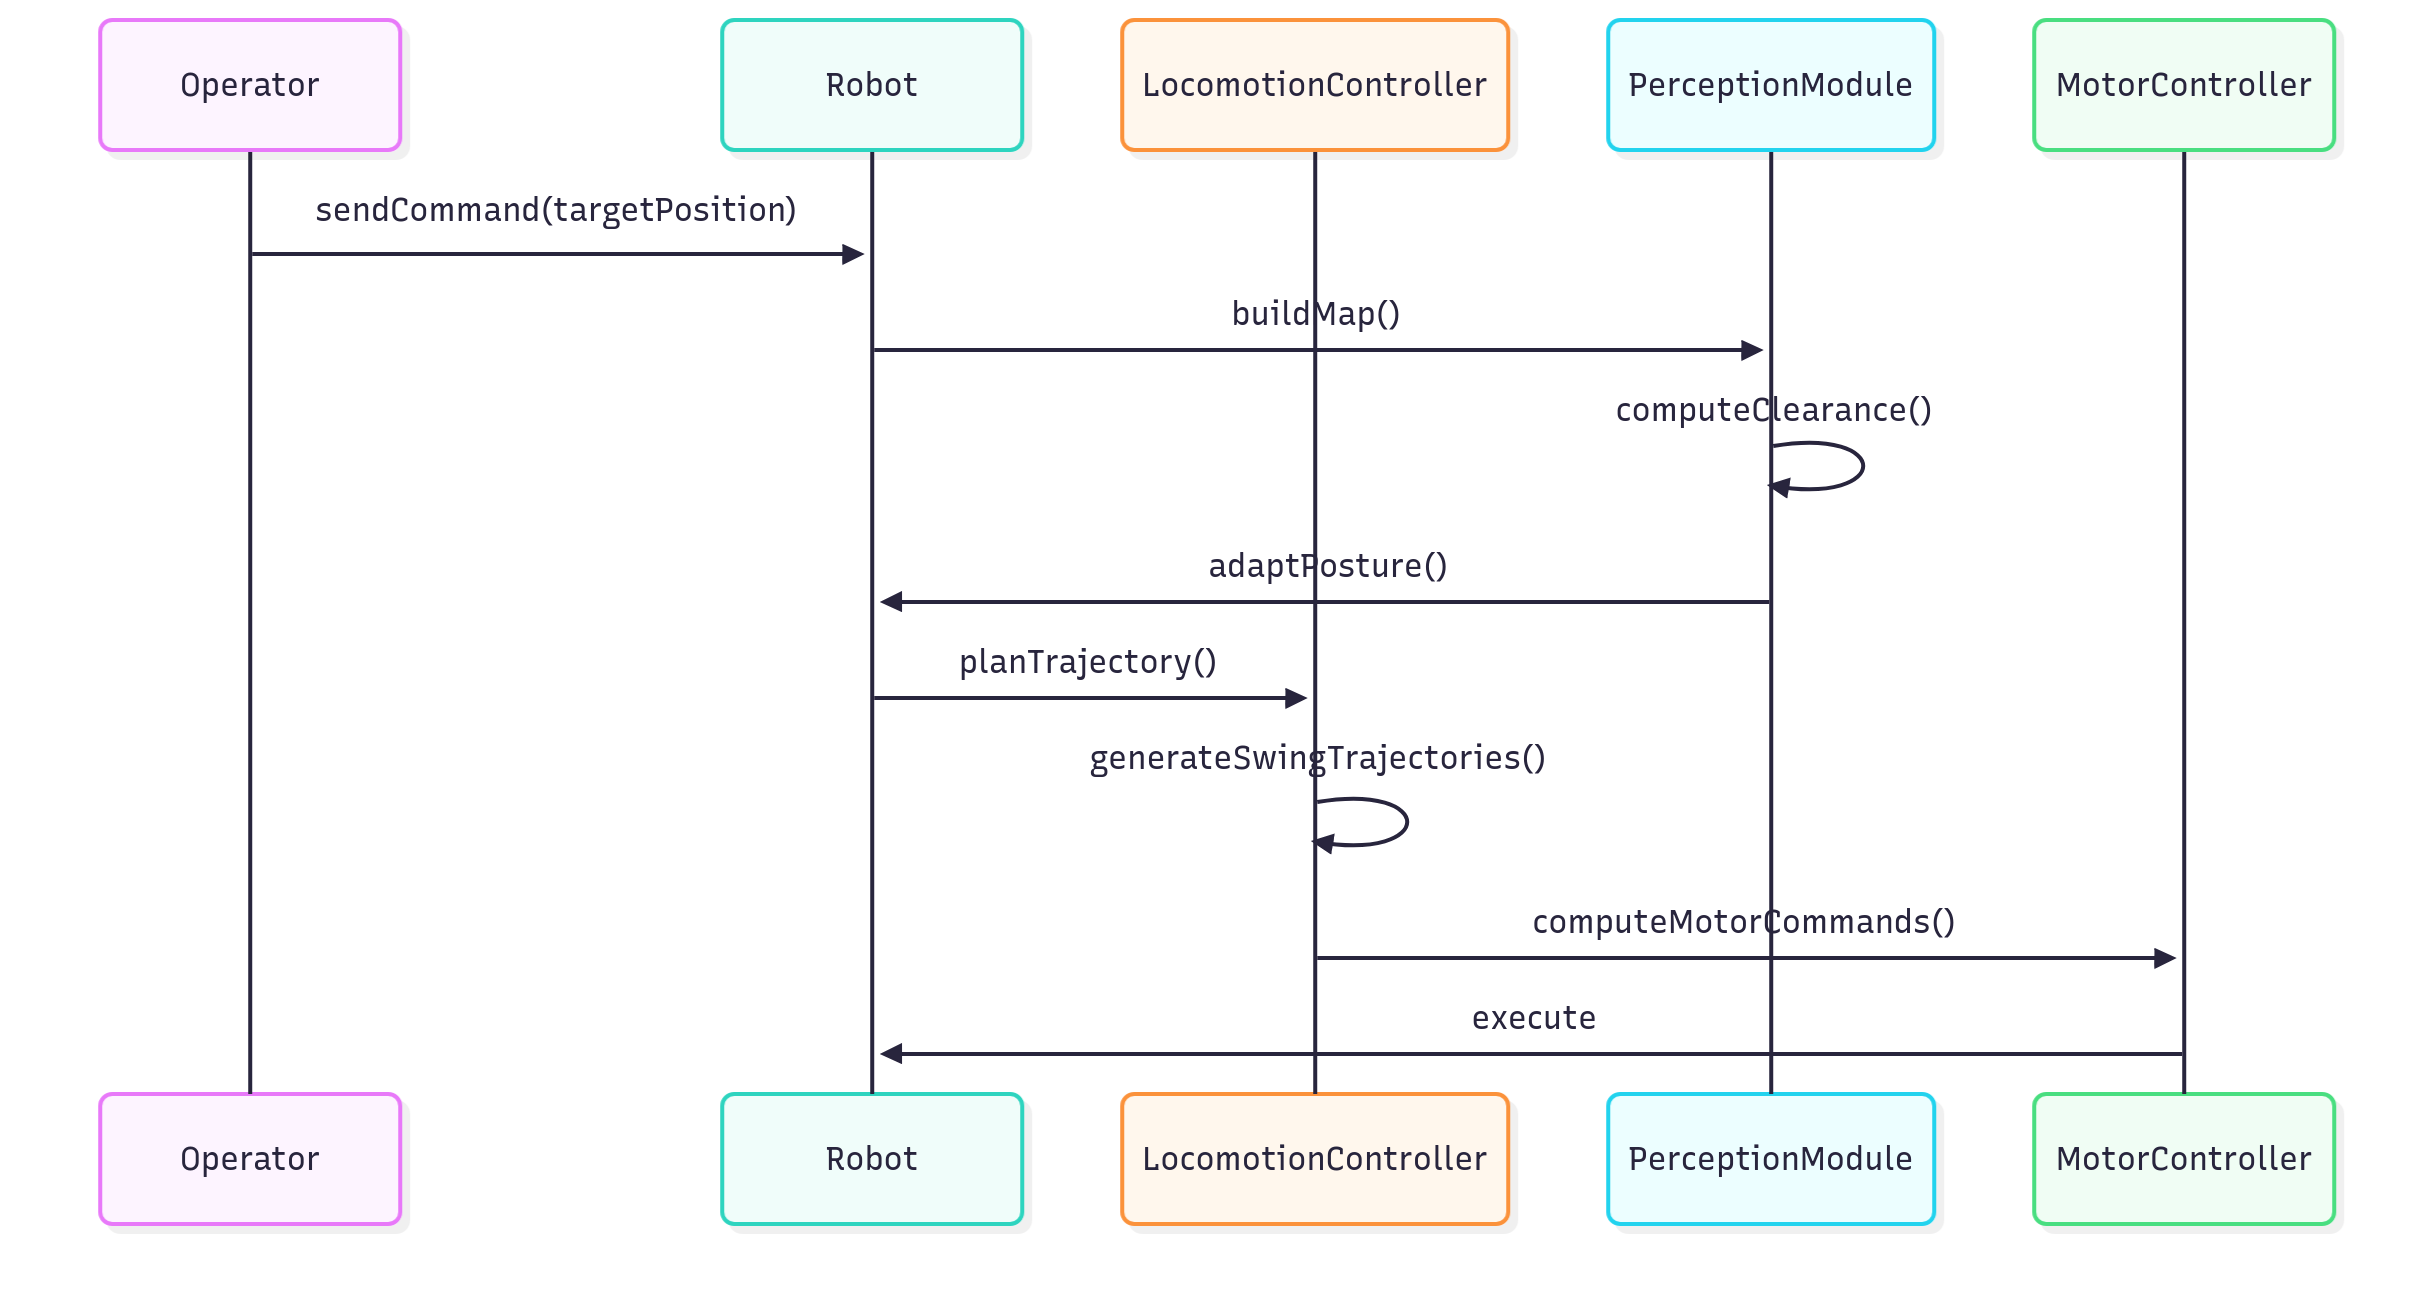
\includegraphics[width=1.0\textwidth]{locomotion.png}
    \caption{Sequence Diagram for the Locomotion Pipeline, detailing the interaction between the operator, robot, and core control modules.}
    \label{fig:locomotion_diagram}
\end{figure}

\begin{figure}[h!]
    \centering
    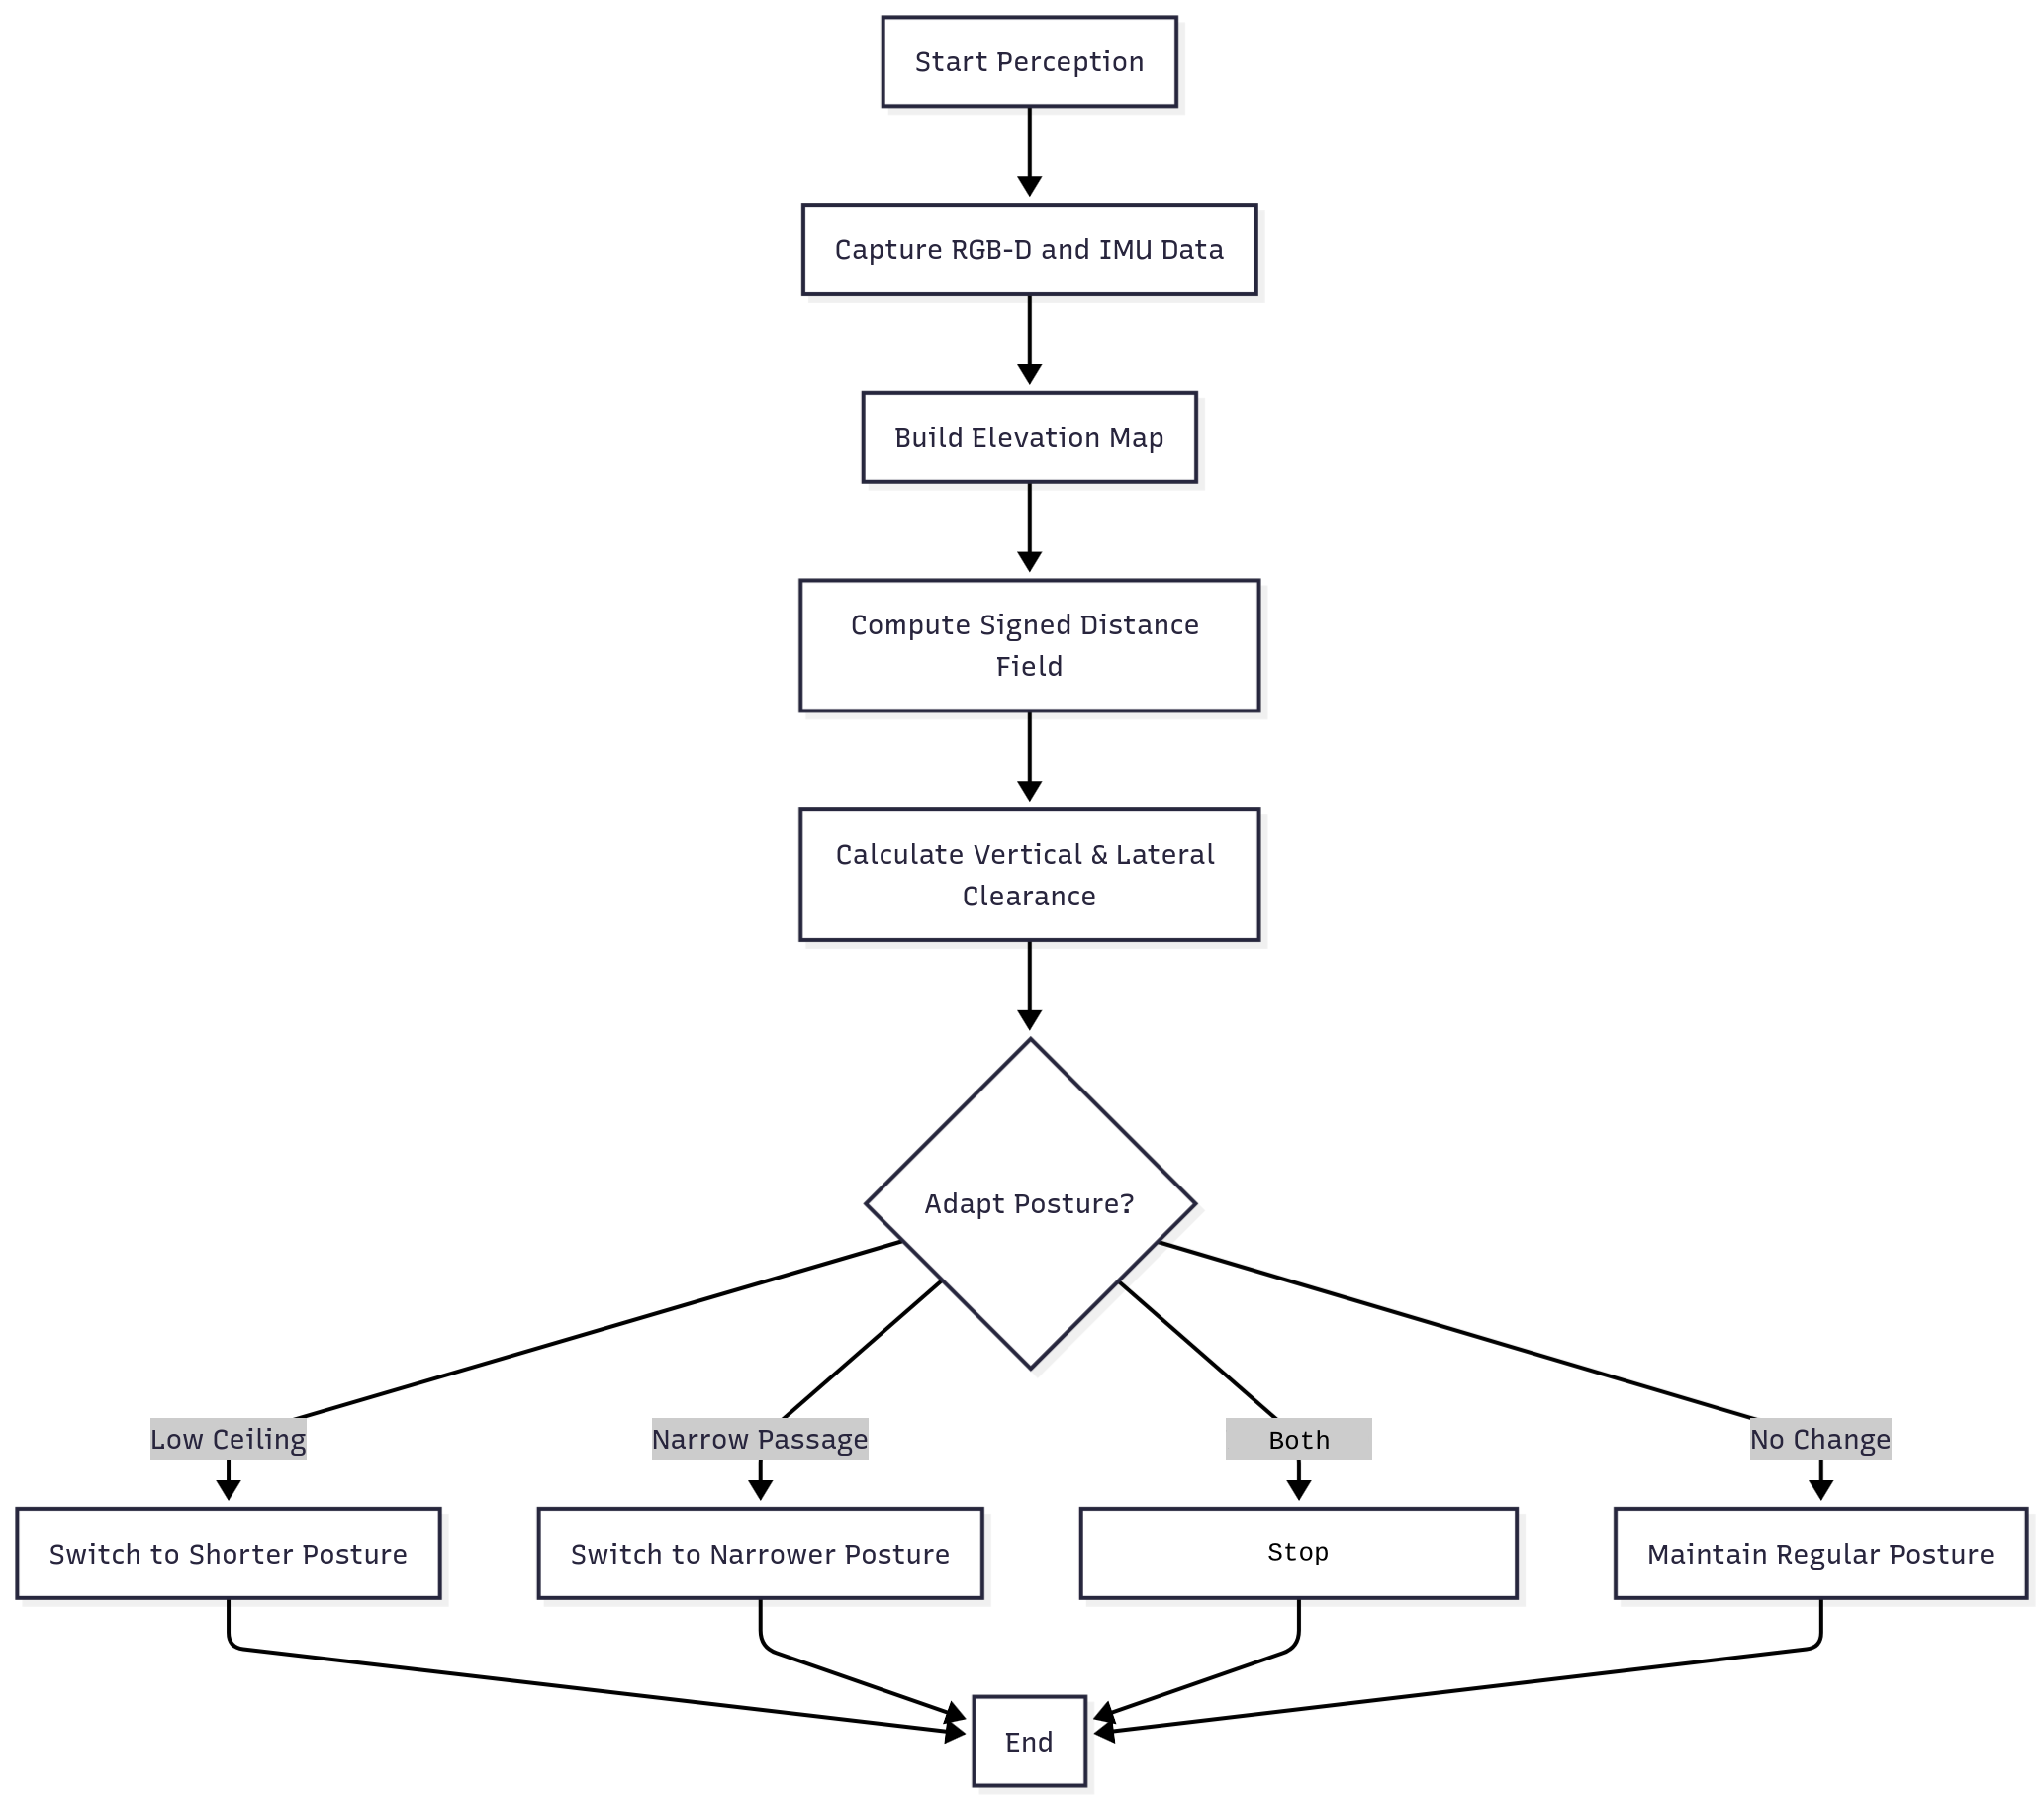
\includegraphics[width=0.8\textwidth]{perception.png}
    \caption{Flowchart for the Perception Pipeline, illustrating the steps from data capture to posture adaptation decision.}
    \label{fig:perception_diagram}
\end{figure}

\begin{figure}[h!]
    \centering
    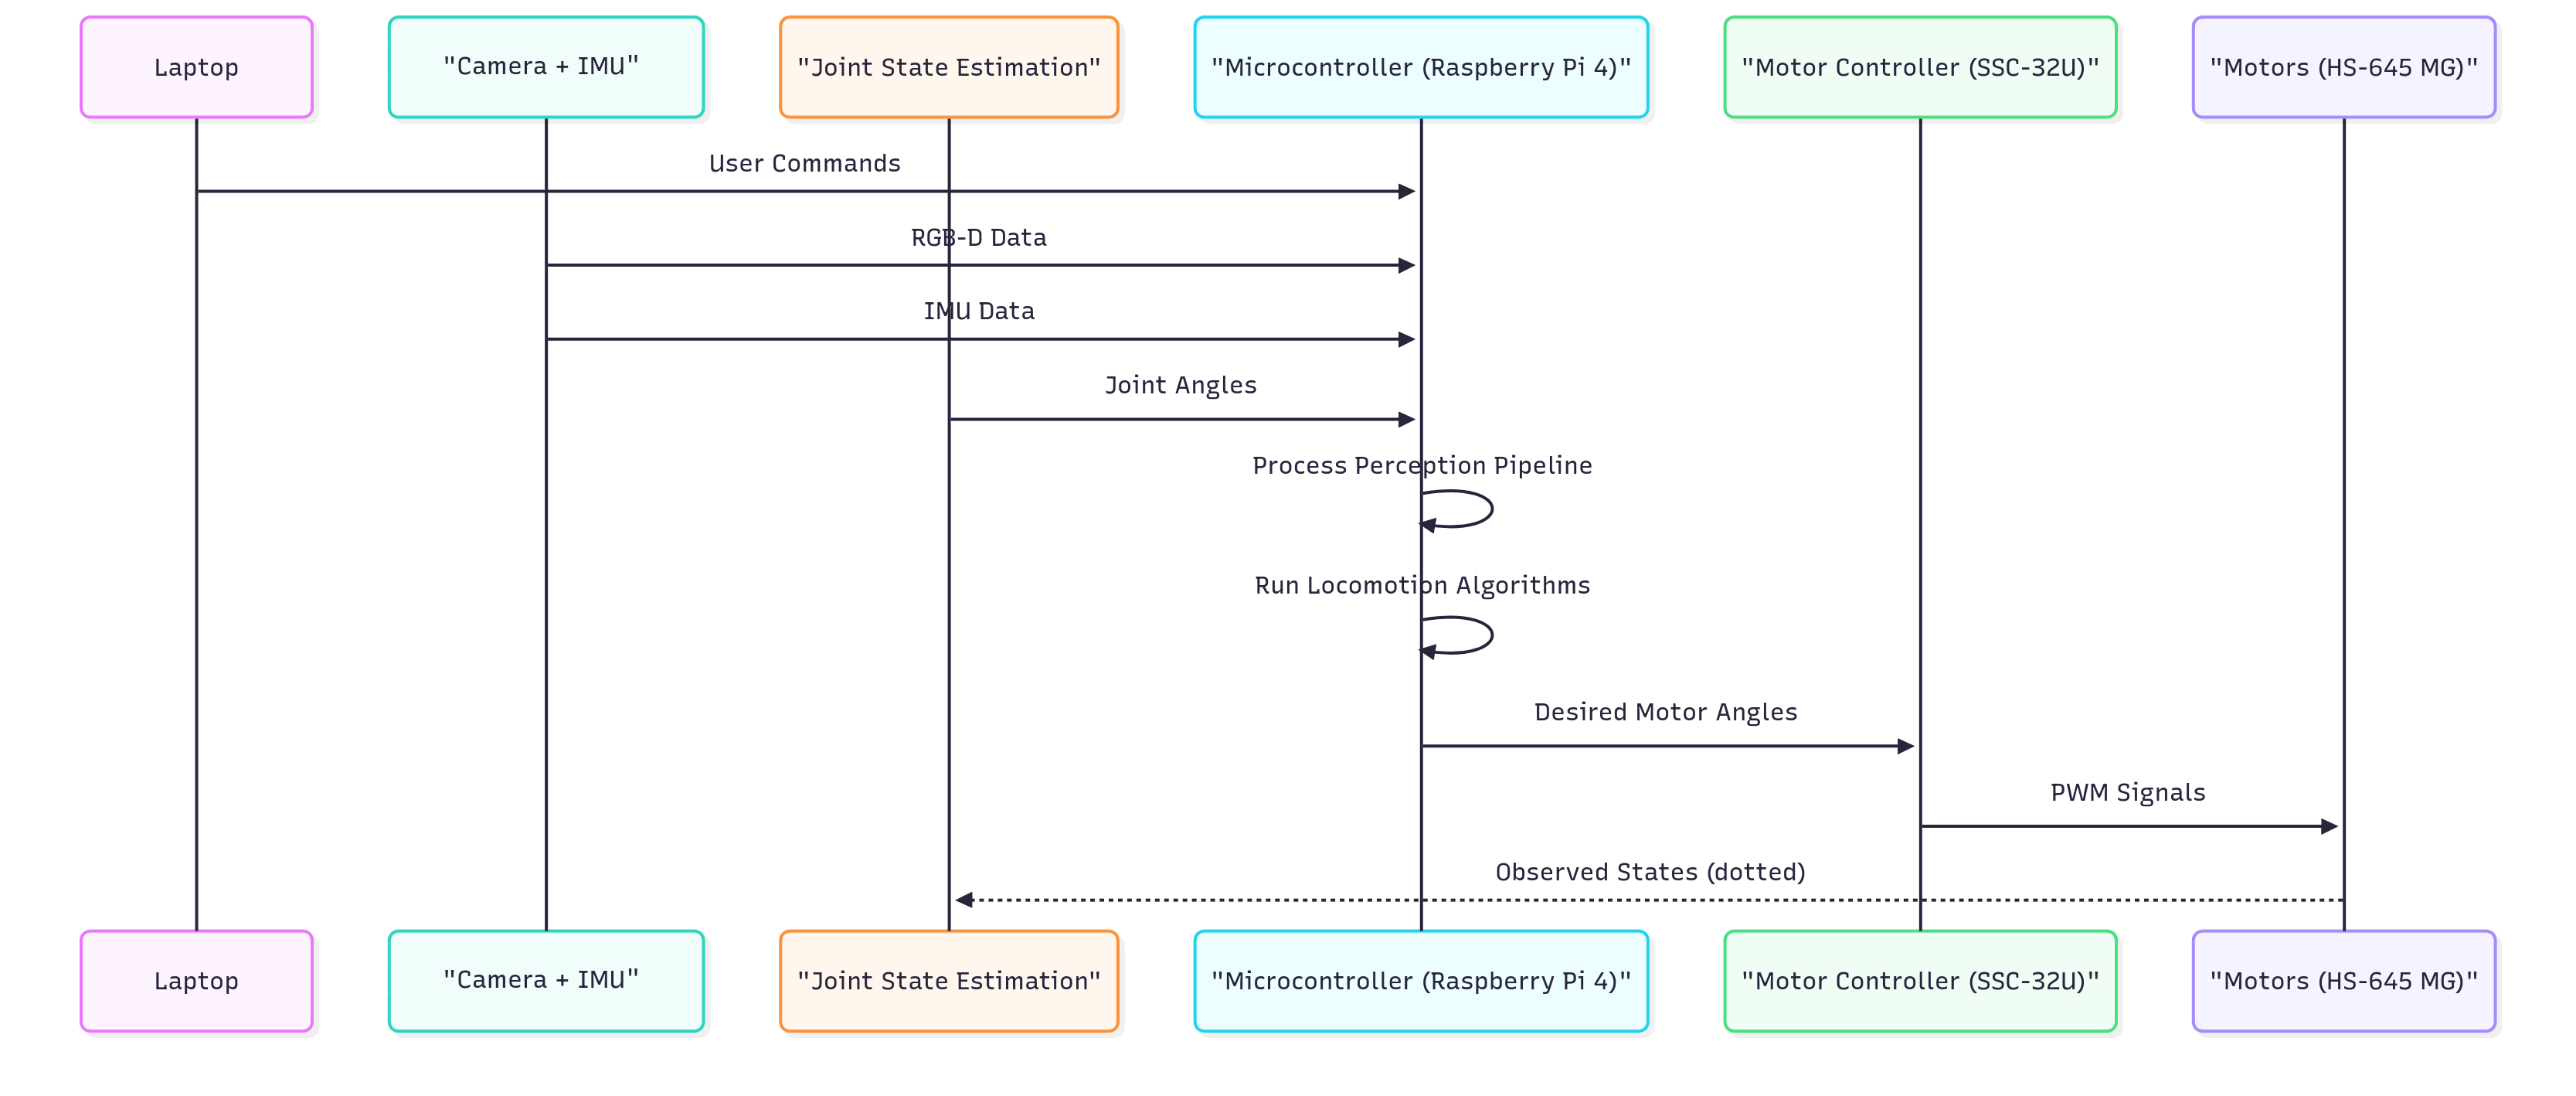
\includegraphics[width=1.0\textwidth]{hardware.png}
    \caption{Sequence Diagram for the Hardware Pipeline, showing the flow of data and commands between physical components.}
    \label{fig:hardware_diagram}
\end{figure}

\section{Technical Details}

Here, we discuss algorithms. Further information is provided in the Robot Technical Document.

The Trajectory Planning Algorithm handles movement. Using Model Predictive Control (MPC), it processes user commands and robot state, returning Center-of-Mass trajectories, leg forces, and swing trajectories. This is to traverse rough terrain.

Next, the  Map Building Algorithm is to build the map from raw RGB-D camera data and IMU readings, applying point cloud processing and odometry correction to generate a $2\text{D}$ elevation map for finding clearance. Essentially, points are classified to floor and ceiling based on their position with regards to the camera frame.

The Posture Adaptation Algorithm reads the elevation map and signed distance field to dynamically adjust the posture:

     Shorter: For low ceilings.
     
     Narrower: For thin gaps.

    Both: Stop.
Else no change from previous state.

The Environment Generation Algorithm uses random procedural generation based on user parameters aforementioned to create rough terrains for simulation.

The microcontroller converts movement commands from locomotion into final PWM signals sent directly to the motors.



\chapter{Methodology, Experiments and Results}
\label{chap:results}
\section{Methodology and Experiments}

The T-Hex kit, as the name suggests, is originally a hexapod. However, due to hardware failures present in our kit, the two middle legs had to be taken out, making it a quadruped. As we wish to eventually extend this work on hardware, we treated the robot as a quadruped. Going forth, T-Hex refers to this quadruped version of the original kit as seen in figure \ref{fig:tquad}. 

\begin{figure}[h]
    \centering
    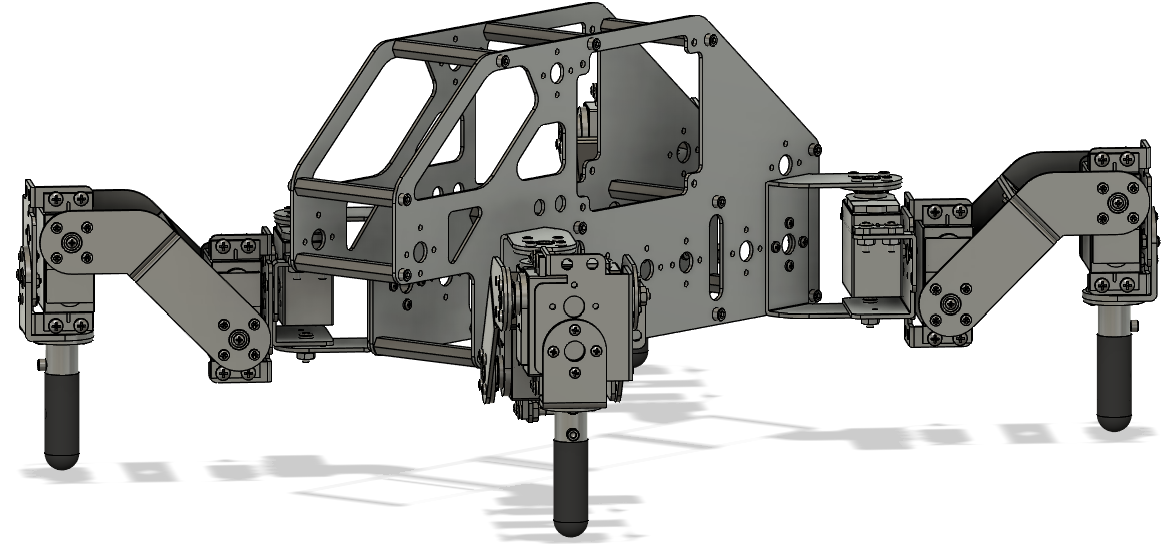
\includegraphics[width=0.7\linewidth]{tquad.png}
    \caption{T-Hex (as seen in SolidWorks) with its middle legs removed, making it a quadruped.}
    \label{fig:tquad}
\end{figure}

\subsection{Kinematics}

The motors of the T-Hex take position commands, that is what angle they should move to, as opposed to torque commands which are common in high-end motors \cite{bledtMITCheetah32018, hutterANYmalHighlyMobile2016}. Each leg of T-Hex has 3 motors (or joints), at the hip, knee, and ankle. Many locomotion controllers, such as an open-loop kinematic gait, output the position of the foot, that is the end point of the legs, at any given time. The problem of determining what joint positions result in a desired foot position is known as the Inverse Kinematics (IK) problem. Solving the IK of a legged robot is well-established. Using the Denavit-Hartenberg (DH) convention, frames of reference are assigned across the robot's legs and the homogenous transform matrices can be multiplied to obtain equations that take in joint positions and output resulting foot positions, known as the Forward Kinematics (FK) equations. The FK equations can then be used to derive the IK equations, that take in foot positions and output the corresponding joint angles. A detailed derivation is omitted for the sake of brevity, but a similar derivation can be found in \cite{sunHexapodRobotKinematics2017}. The IK equations for our robot are as follows:
\begin{align}
    \theta_1 &= \text{atan2}(y, x) \\
    \theta_2 &= 
    \begin{cases} 
        \arcsin\left(\frac{z}{a_2}\right) + \phi_2 & \text{for right legs} \\
        \arccos\left(\frac{z}{a_2}\right) - \phi_2 & \text{for left legs}
    \end{cases} \\
    \theta_3 &= 
    \begin{cases} 
        \frac{\pi}{4} & \text{for right legs} \\
        -\frac{\pi}{4} & \text{for left legs}
    \end{cases} \\
    \theta_4 &= 
    \begin{cases} 
        \phi_1 - \arcsin\left(\frac{\Psi}{a_1}\right) & \text{for right legs} \\
        -\arccos\left(\frac{\Psi}{a_1}\right) - \phi_1 & \text{for left legs}
    \end{cases} 
\end{align}

where $\Psi, a_1, \phi_1 a_2,$ and $\phi_2$ are defined as:
\begin{align}
    \Psi &= \frac{1}{2L_4} \Big[ (x \cos\theta_1 + y \sin\theta_1 - L_1)^2 + z^2 \notag \\
    &\quad - L_2^2 - L_3^2 - L_4^2 - 2L_2 L_3 \cos\theta_3 \Big] \\
    A_1 &= L_2 \cos\theta_3 + L_3 \\
    B_1 &= L_2 \sin\theta_3 \\
    a_1 &= \sqrt{A_1^2 + B_1^2} \\
    \phi_1 &= 
    \begin{cases} 
        \text{atan2}(A_1, B_1) & \text{for right legs} \\
        \text{atan2}(B_1, A_1) & \text{for left legs}
    \end{cases} \\
    A_2 &= L_2 + L_3 \cos\theta_3 + L_4 \cos(\theta_3 + \theta_4) \\
    B_2 &= L_4 \sin(\theta_3 + \theta_4) + L_3 \sin\theta_3 \\
    a_2 &= \sqrt{A_2^2 + B_2^2} \\
    \phi_2 &= 
    \begin{cases} 
        \text{atan2}(B_2, A_2) & \text{for right legs} \\
        \text{atan2}(A_2, B_2) & \text{for left legs}
    \end{cases}
\end{align}

where $x, y,$ and $z$ are input foot coordinates in the \textit{hip frame} of the leg and $L_i$ indicates the length of the $i$-th link. While each leg in the T-Hex has only 3 motors, it has a $45$ degree bend in between the knee and ankle motors (as can be seen in figure \ref{fig:tquad}) which we model as a rigid joint (see eq. (3)); hence, we have four links.


\subsection{Simulation}

To simulate the robot, we used the available CAD model (as seen in figure \ref{fig:tquad}) and the SolidWorks plugin SW2URDF \cite{Sw_urdf_exporterROSWiki} to export a URDF file for simulating the robot. Certain properties, such as mass and inertia, were exported incorrectly and had to be manually adjusted using calculations from SolidWorks. Furthermore, we also made a simplified collision mesh to be used in place of the high fidelity CAD model to speed up simulation. We used Gazebo Sim as our primary simulator.

To simulate terrain, we had two types of terrains: a flat world with some narrow passageways and crawl spaces made out of cuboids, and a rough terrain cave procedurally generated via modifying PLUME \cite{garciaPLUMEProceduralLayer2025}, a procedural cave generation framework, for our lava tube case. In both terrains, the ground's friction coefficient was set to 0.7.

\begin{figure}[h]
    \centering
    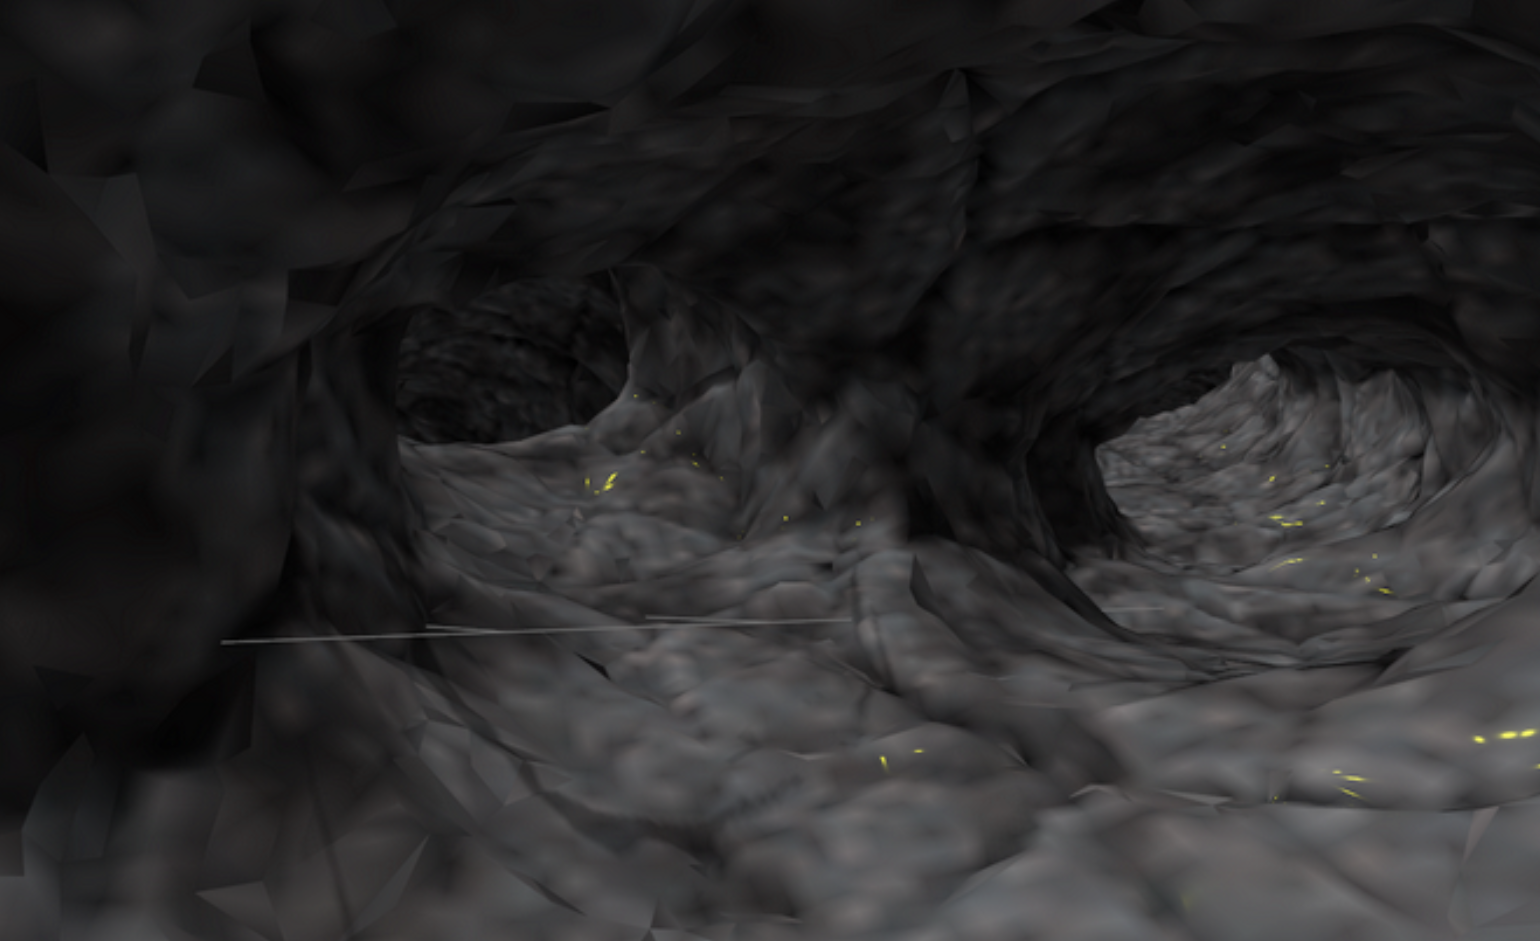
\includegraphics[width=0.8\linewidth]{cave.png}
    \caption{Interior of cave generated using PLUME \cite{garciaPLUMEProceduralLayer2025}}
    \label{fig:cave}
\end{figure}

After simulating the robot and terrains to test our locomotion controllers in, we set out to work on the locomotion controllers themselves. To cover both model-free and model-based controllers, we worked on the following three controllers:
\begin{enumerate}
    \item An \textbf{open-loop kinematic gait} to serve as a baseline for walking in flat terrain
    \item A \textbf{deep reinforcement learning} based controller trained in Isaac Lab 
    \item A \textbf{model-based controller} based off of MIT Cheetah 3's locomotion controller \cite{bledtMITCheetah32018}
\end{enumerate}

In simulation, the work on perception was taken separately, with the goal of giving posture signals that could be sent to the above controllers. 

\subsection{Open-loop kinematic gait}

For this controller, we use a crawl gait. For a quadruped, a crawl gait is one where at most one leg is in swing phase at a given time, giving a wider support polygon under the robot with three legs in stance. Hence, the stance phase is three times longer than the swing phase. The different permutations for the swing legs may result in better or worse stability. Typically, alternating sides (left and right) in the swing order helps keep the robot from tilting too far on one side. A possible schedule is given in table \ref{tab:crawl_gait}. 

\begin{table}[h]
    \centering
    \caption{Crawl Gait Schedule}
    \label{tab:crawl_gait}
    \newcolumntype{Y}{>{\centering\arraybackslash}X} 
    
    % \columnwidth ensures it spans exactly the width of the IEEE column
    \begin{tabularx}{\columnwidth}{@{}lYYYY@{}}
        \toprule
        \textbf{Leg} & \textbf{$0 \le t < \frac{N}{4}$} & \textbf{$\frac{N}{4} \le t < \frac{N}{2}$} & \textbf{$\frac{N}{2} \le t < \frac{3N}{4}$} & \textbf{$\frac{3N}{4} \le t < N$} \\
        \midrule
        FR & \cellcolor{white} Swing & \cellcolor{gray!30} Stance & \cellcolor{gray!30} Stance & \cellcolor{gray!30} Stance \\
        BL & \cellcolor{gray!30} Stance & \cellcolor{white} Swing & \cellcolor{gray!30} Stance & \cellcolor{gray!30} Stance \\
        BR & \cellcolor{gray!30} Stance & \cellcolor{gray!30} Stance & \cellcolor{white} Swing & \cellcolor{gray!30} Stance \\
        FL & \cellcolor{gray!30} Stance & \cellcolor{gray!30} Stance & \cellcolor{gray!30} Stance & \cellcolor{white} Swing \\
        \bottomrule
    \end{tabularx}
\end{table}


We pre-compute trajectories of $N$ discrete foot positions for each leg. A normalized phase variable $\tau \in [0, 1]$ dictates how far along a leg is in either swing or stance phase (based on the gait schedule). In swing phase, a quadratic bezier curve is used to generate trajectory points whereas in stance phase, linear interpolation between the start and end points of the swing phase can be used.

\begin{align}
    \mathbf{p}_{swing}(\tau) &= 
    \begin{bmatrix} 
        X \\ 
        (1-\tau)^2 P_{y} + 2(1-\tau)\tau Q_{y} + \tau^2 R_{y} \\ 
        (1-\tau)^2 P_{z} + 2(1-\tau)\tau Q_{z} + \tau^2 R_{z} 
    \end{bmatrix} \\
    \mathbf{p}_{stance}(\tau) &= 
    \begin{bmatrix} 
        X \\ 
        \frac{T}{2} (1 - 2\tau) \\ 
        S 
    \end{bmatrix}
\end{align}

where $X$ is the longitudinal distance from the hip (the sprawl of the robot), $S$ is the vertical distance from the hip (how far above the ground the robot stands), $T$ is the total distance covered in the stance phase, and $P = [X,-T/2, S]^T, Q = [X,0, S + 2A]^T,$ and $R = [X,T/2, S]^T$ are the control points of the bezier curve, where $A$ is the amplitude of the swing phase (how far above the ground is the apex of the swing). To make the generated trajectories parallel to the length of the robot, the trajectories for each leg were rotated by the angle corresponding to the offset of the corresponding hip frame in zero position (the hip motor at zero degrees) from the frame placed at the center of the robot.

\begin{figure}[h]
    \centering
    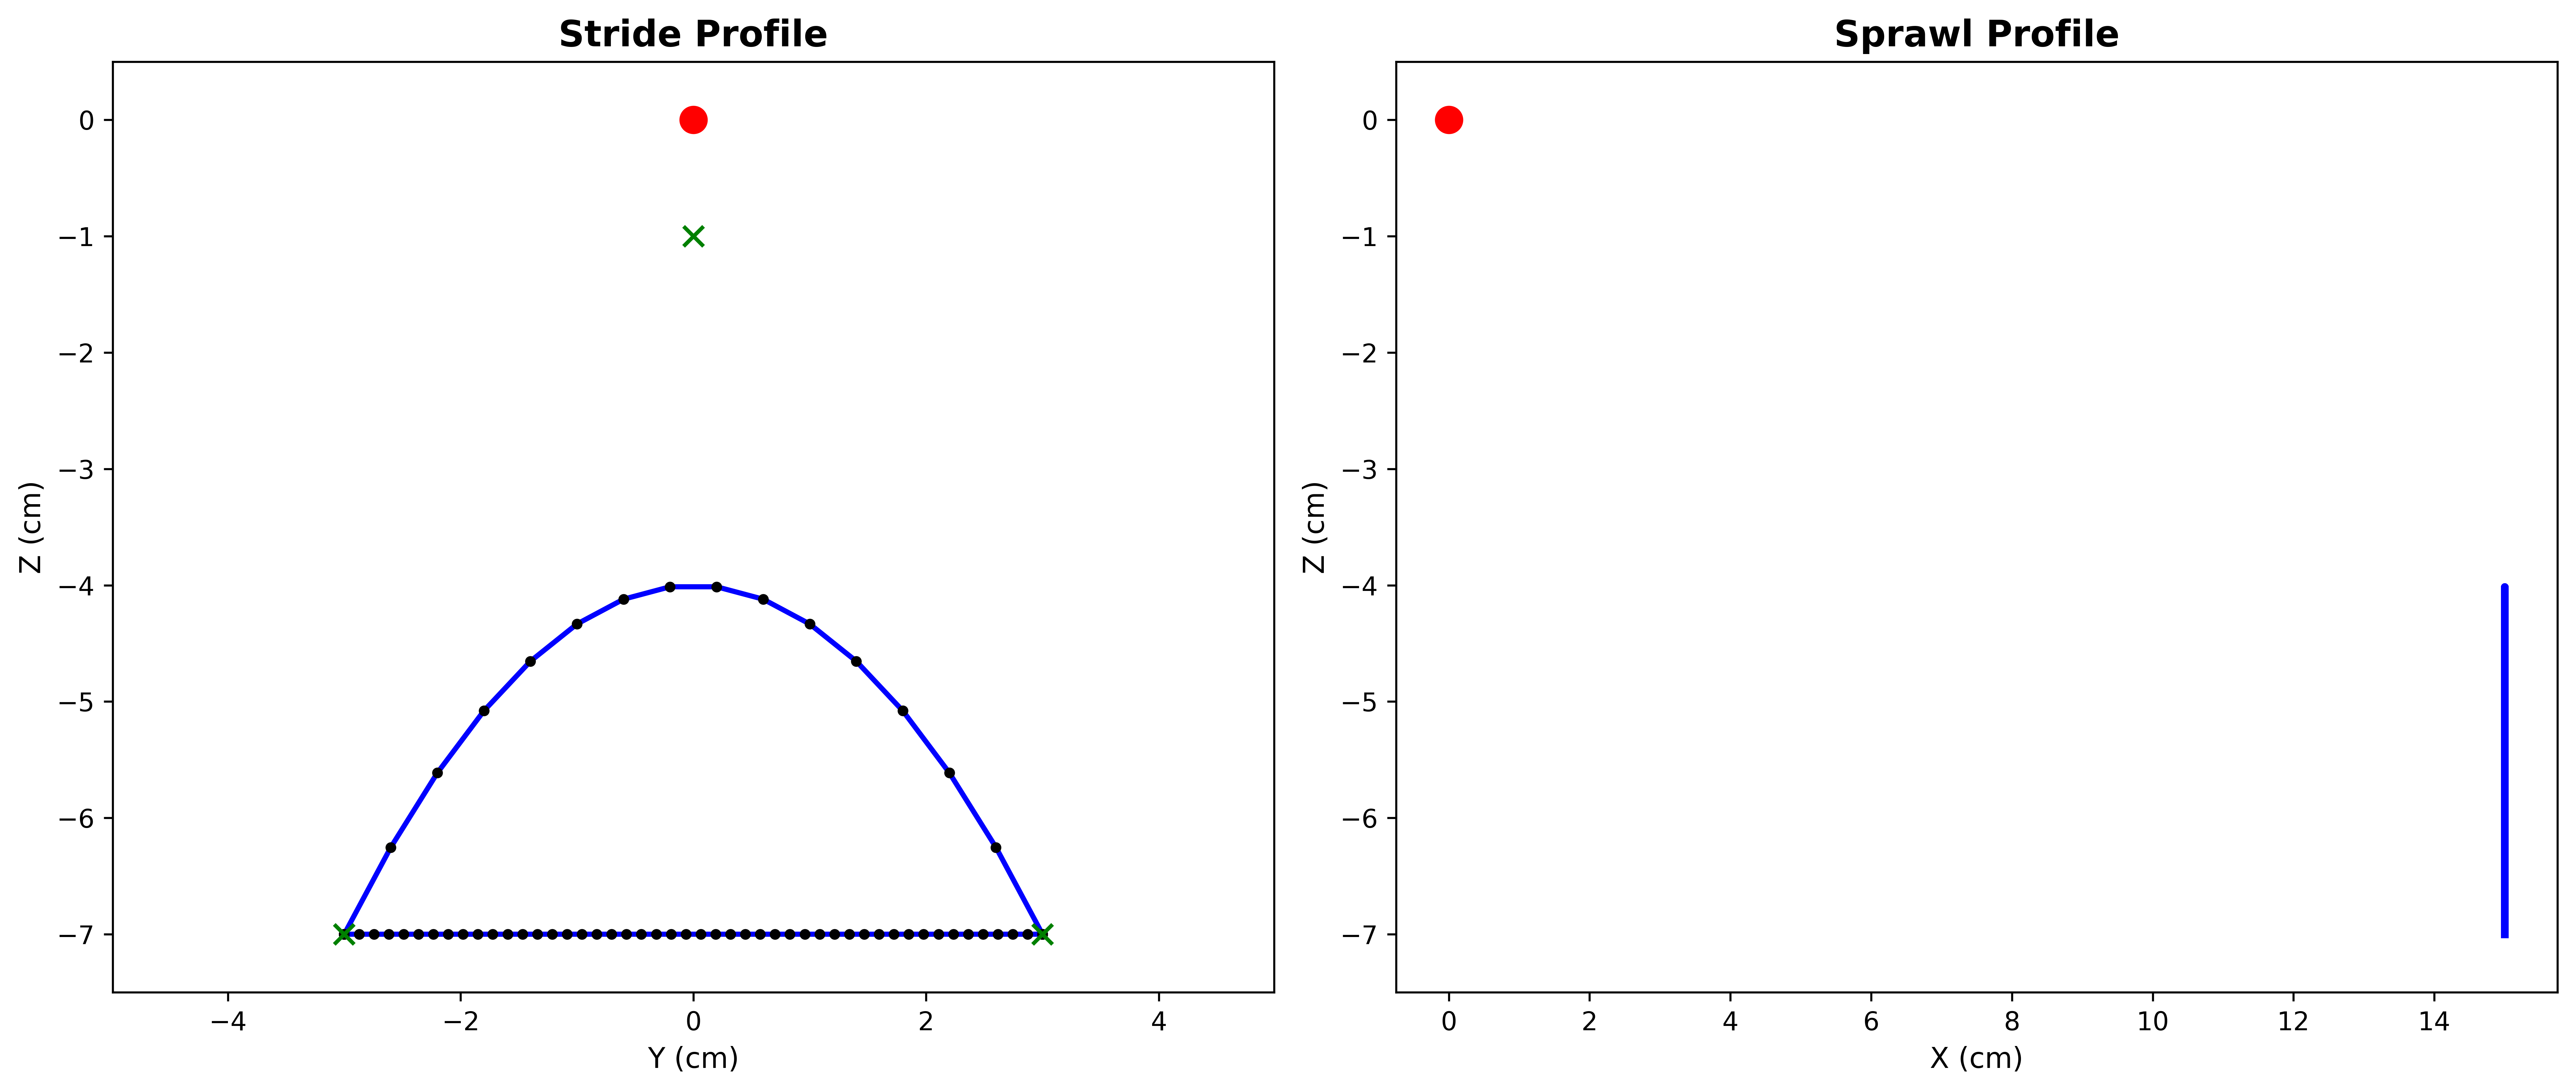
\includegraphics[width=\linewidth]{foot_trajectory_combined.png}
    \caption{Visualization of Bezier Curve with $N = 64, X = 15, S = -7, A = 3, T = 6$ in the hip's Y-Z plane (left) and X-Z plane (right). The red point indicates the location of where the hip frame was placed. The green crosses (in the left plot) indicate the bezier curve control points $P$, $Q$, and $R$.}
    \label{fig:gait}
\end{figure}

\subsection{Deep Reinforcement Learning-based Controller}

To train a DRL-based controller, we used Isaac Sim to convert the robot's URDF into an USD file. Then, we used a pre-existing Isaac Lab setup for velocity tracking for ANYmal C and modified it for our use case. 4096 instances of T-Hex \footnote{Other hyperparameters were kept the same as \cite{rudinLearningWalkMinutes2022}} were spawned in an environment containing three different categories of terrains: random noise rough terrain created using grids of points of varying heights connected together with planes, random blocks rough terrain consisting of flat blocks of varying heights arranged in a grid, and random inclines created by taking the maximum and minimum of planes of varying slopes. The maximum vertical distance between any two points in the random noise rough terrain was set to 6cm, the maximum vertical distance between adjacent blocks in random blocks rough terrain was set to 3cm, and the slope of the planes in random inclines was between -15 and 15 degrees. However, as is typical in literature \cite{rudinLearningWalkMinutes2022, rudinAdvancedSkillsLearning2022, hoellerANYmalParkourLearning2023}, instead of spawning all robots at the highest end of the difficulty for each category, a curriculum learning approach was adopted where the robots would spawn in easier difficulty variants of each category, and advance to higher difficulties after successfully performing at the lower difficulty. Further details regarding the setup can be found in \cite{rudinLearningWalkMinutes2022}.

The input to the policy network was the robot's current joint positions, the projected gravity vector (the gravity vector in robot's base frame), its angular velocity, previous actions given by the policy, and the user commands for $xy$-linear velocity and $z$-angular velocity (yaw rate). The network's output was joint commands for each of the twelve joints. The value network was given all the same inputs as the policy network, along with some privileged information to speed up training, such as joint velocities, robot's base linear velocity, and the height values of 128 random points on the terrain around the robot.

Table~\ref{tab:rl_rewards} lists the rewards and penalties used during training along with their weights.

\begin{table}[h!]
    \centering
    \caption{Rewards and Penalties for Training DRL-based Controller}
    \label{tab:rl_rewards}
    % \newcolumntype defines a centered X column to stretch the math evenly
    \newcolumntype{C}{>{\centering\arraybackslash}X}
    \begin{tabularx}{\columnwidth}{@{} >{\raggedright\arraybackslash}p{2.8cm} C c @{}}
        \toprule
        \textbf{Reward/Penalty} & \textbf{Calculation} & \textbf{Weight} \\
        \midrule
        XY-Linear Velocity Tracking & $\exp\left(-\frac{\|\mathbf{v}_{xy} - \mathbf{v}_{xy}^{cmd}\|^2}{\sigma}\right)$ & 3 \\
        \addlinespace
        Z-Angular Velocity Tracking & $\exp\left(-\frac{(\omega_z - \omega_z^{cmd})^2}{\sigma}\right)$ & 1 \\
        \addlinespace
        Feet Air Time & $\sum_{foot} \max(0, t_{air} - 0.1)$ & 2 \\
        \addlinespace
        Z-Linear Velocity Tracking & $-v_z^2$ & -2 \\
        \addlinespace
        XY-Angular Velocity Tracking & $-(\omega_x^2 + \omega_y^2)$ & -0.05 \\
        \addlinespace
        Action Rate & $-\|\mathbf{a}_t - \mathbf{a}_{t-1}\|$ & -0.01 \\
        \addlinespace
        Joint Torques & $-\sum_i \tau_i^2$ & -1e-6 \\
        \addlinespace
        Joint Accelerations & $-\sum_i \ddot{q}_i^2$ & -2.5e-7 \\
        \addlinespace
        Undesired Contacts & $-\sum \mathbb{I}(\text{contact})$ & -1 \\
        \bottomrule
    \end{tabularx}
\end{table}

\subsection{MIT Cheetah 3-like Controller}

Heavily inspired by the MIT Cheetah \cite{bledtMITCheetah32018} control architecture and its implementations \cite{mit_cheetah_github, shuo_yang_github, pympc_github}, we have implemented a similar controller, albeit with some changes according to our structure and limitations.

% \begin{figure}[htbp]
% \centerline{\includegraphics[width=0.5\textwidth]{MITcheetah.png}}
% \caption{MIT Cheetah 3 }
% \label{cheetah}
% \end{figure}

At the highest level, the user gives commands for desired linear and angular velocity of the robot's base. The controller is responsible for generating torque commands for the stance and swing legs, which are decided base on the gait schedule. 

For the gait schedule, we implemented the crawl gait implementation taken from \cite{shuo_yang_github} which publishes the nominal schedule for all legs, along with the swing and stance times for each leg and how much of each state has been completed by a leg. This information, along with state feedback, is passed to an FSM which determines early contacts only, as opposed to \cite{bledtMITCheetah32018} determining both early and late contacts. The current state of each leg is published and this information is utilized by the stance and swing controllers. 

The stance controller first computes the desired COM position based on the virtual support polygon approach. It then uses this along with the robot state, inertia and constant weight parameters to implement a PD controller, called the Balance Controller by the authors. The dynamics model described in their paper has a simplification of massless legs, which is applicable for robots such as the MIT Cheetah 3, but to THex. Still, to accurately follow the architecture, we have implemented their dynamics model entirely, and used that in the balance controller to calculate the forces needed to support the robot in stance. These forces need to be computed through a convex optimization solver, for which we used OSQP \cite{osqp}.

The swing controller makes use of the robot state and other control parameters to calculate the foot trajectory and determine where the feet should be placed. We have used the approach described in \cite{bledtMITCheetah32018} to calculate the final foot position and generated a bezier curve trajectory to reach that point. The foothold calculation used by the authors works well for dog-like robots as it places the foothold on the ground right ahead of the hip frame; however, for robots like the T-Hex, the footholds need to be offset from the hip. We used a constant for this offset. Since the legs are in swing and do not require extensive optimization to find optimal forces, we have used the PD controller described by the authors. The stance and swing forces are then converted to torque commands and sent to the appropriate legs.

\subsection{Posture Adaptation}

Inspired by \cite{buchananWalkingPostureAdaptation2019}, the essential purpose of this pipeline was that, given raw depth data of the environment, output body configurations with a height $Z^*$ and  and corresponding leg span $S^*$ which best keep the robot away from collisions in confined spaces.

First, the camera creates a pointcloud of the local environment. This is essentially an RGB image where each pixel has an XYZ coordinate associated to it depending on its location in real life, hence creating a cloud of points. First, these points are projected onto an XY grid and split in half depending on camera height. Each half is run through the grid map algorithm by Fankhauser et al. \cite{fankhauserRobotcentricElevationMapping2014}, creating a a \textit{floor}
layer $F(x,y)$ and a
\textit{ceiling} layer $C(x,y)$.
Next, for every cell, the available vertical headroom is:
\begin{equation}
    h_{avail}(x, y) = C(x, y) - F(x, y)
\end{equation}

Now, cells where the headroom falls below the robot's minimum possible
height $z_{min}$ are classified as unsafe for traversal:
\begin{equation}
    W(x, y) = \begin{cases} 1 & \text{if } h_{avail}(x, y) < z_{min} \\ 0 & \text{otherwise} \end{cases}
\end{equation}
Now, to obtain the horizontal legroom per cell to the nearest unsafe region, a Euclidean Distance Transform (EDT) is applied to the wall map :
\begin{equation}
    w_{avail}(x, y) = \left( \min_{(x_w, y_w) \in W} \sqrt{(x-x_w)^2 + (y-y_w)^2} \right) \times \text{res}
\end{equation}
where $\text{res}$ is the map resolution in m/cell.

Now it is appropriate to consider leg span, which we assume is inversely proportional to height and is modeled as:
\begin{equation}
    S(Z) = s_{max} - \left(\frac{Z - z_{min}}{z_{max} - z_{min}}\right)(s_{max} - s_{min})
\end{equation}
where $z_{min}, z_{max}$ are the kinematic height limits and
$s_{min}, s_{max}$ are the corresponding span limits.

We then iterate through each candidate height $Z$ in a discrete set
$\{Z_1, \dots, Z_{15}\}$, and compute the vertical and horizontal safety margins
as follows:
\begin{align}
    M_Z(Z) &= h_{avail}(x, y) - Z \\
    M_W(Z) &= w_{avail}(x, y) - S(Z)
\end{align}
which are then scored accordingly:
\begin{equation}
    \text{Score}(Z) = \begin{cases} \min(M_Z(Z),\, M_W(Z)) & \text{if } Z \leq h_{avail} \text{ and } S(Z) \leq w_{avail} \\ -\infty & \text{otherwise} \end{cases}
\end{equation}
The optimal height has the best score of the lot:
\begin{equation}
    Z^* = \arg\max_{Z}\, \text{Score}(Z)
\end{equation}
and so the corresponding span $S^* = S(Z^*)$ is passed alongside $Z^*$ as
posture commands to the locomotion controller.

\section{Results}

The open-loop kinematic gait was successful in walking in flat terrain, with high sensitivity to the choice of gait parameters as well as the gait schedule. However, it was expectedly poor at walking in rough terrain, often getting stuck when going up hill or falling over when going down hill. Testing the open-loop kinematic gait on hardware gave similar results, with the robot successfully walking in flat terrain. A shortcoming of the open-loop kinematic gait is that any disturbance caused by noise or software or hardware latency causes the robot's heading to deviate, which makes the robot gradually turn while walking.

In simulation, the robot was tested with a camera on posture adaptation for multiple cases: a normal region, a low region, a thin region, and a low and thin region. Based on this, it was successfully able to plot out required postures as per the circumstances and then change its posture before entering the region and in the case of the last region refusing to enter; however, it must be kept in mind that this robot was utilizing a kinematic based gait, which was incapable of turning. Hence, while it could adapt its height, it could not make use of traversability for regions best away from the walls, thus hampering its performance. 

\begin{figure}[htbp]
\centerline{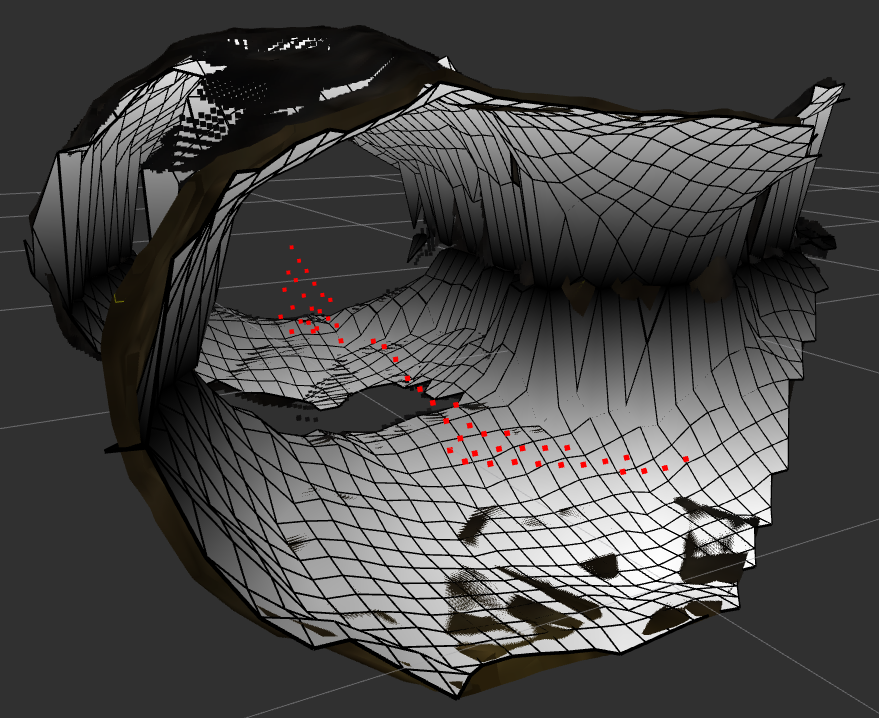
\includegraphics[width=0.5\textwidth]{posture.png}}
\caption{A live cave pointcloud, its mapped floors and ceiling, and best z-values per safe zone. }
\label{posture}
\end{figure}

The DRL-based controller was successful in learning to walk in the random noise rough terrain and random incline terrains up till the highest difficulty, but only learned to walk in the random blocks rough terrain up till 60\% of the highest difficulty. The reason for this is that the random blocks rough terrain can have discontinuities jumps in the terrain's height, which can be difficult to learn to walk in for a proprioceptive controller that cannot perceive the terrain. When the DRL-based controller was tested in the cave generated by PLUME, it was able to traverse it, but required careful teleoperation to find the right path to take. 

\begin{figure}[htbp]
\centerline{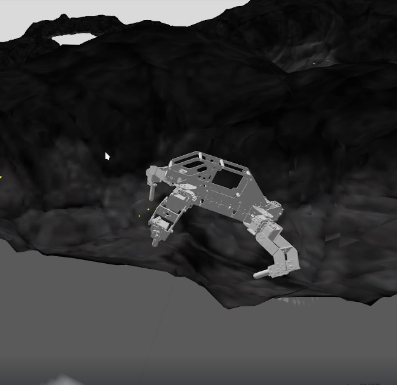
\includegraphics[width=0.5\textwidth]{example.png}}
\caption{Snapshot of the robot walking in the simulated cave. }
\label{example}
\end{figure}

The MIT Cheetah 3-like controller did not perform well in even flat terrain. The robot would not be able to lift its legs off the ground to take a step, often shuffling its feet on the ground and not making much forward progress. A suspected reason for this is that the controller uses a simplified dynamic model of the robot that assumes the robot's legs are massless, which is not the case for T-Hex. Furthermore, our modification to the foothold planning also restricts the sprawl of the robot, which could be chosen dynamically to help the robot balance itself better. 



\chapter{Conclusion and Future Work}
\label{chap:outro}
We modeled the kinematics of the T-Hex kit and created a simulation package for testing locomotion controllers. We implemented three different controllers, along with a posture adaptation pipeline that gives the nominal base height for locomotion. We integrated the posture adaptation pipeline with the open-loop kinematic gait and tested it in flat terrain and found success in navigating confined spaces. However, the open-loop kinematic gait was expectedly poor at walking in rough terrain. The DRL-based controller was successful in learning to walk in rough terrain, albeit with some limitations in the random blocks rough terrain. The MIT Cheetah 3-like controller did not perform well, likely due to the assumptions made in the dynamic model used for control. 

Our next steps include integrating the posture adaptation pipeline with the DRL-based controller, building upon the MIT Cheetah 3-like controller to adapt it for our robot, and testing the DRL-based controller and the MIT Cheetah 3-like controller in hardware. To integrate the posture adaptation pipeline with the DRL-based controller, we plan on training three separate policies for three different nominal base heights, and then use the posture adaptation pipeline to determine which nominal base height to use at any given time. To adapt the MIT Cheetah 3-like controller for our robot, we plan on looking into more accurate dynamic models that take into account the mass of the legs, as well as more robust approaches to foothold selection. Furthermore, as the controller generates torque commands, we also plan to adapt the controller to convert torque commands into position commands \cite{zepedaTheoreticalConversionTorque2024,delpreteImplementingTorqueControl2016,khatibTorquepositionTransformerTask2008} so that it can be tested on hardware.

\chapter{Reflection}
\label{chap:Reflection}
Learning Reflection: This was another bachelor degree's worth of learning in itself. On the skills side of things, we learned how to practically apply kinematics, reinforcement learning, robot perception, environment simulation, and so many more topics to a real, tangible problem. Aside from that, we had to familiarize ourselves extensively with novel softwares and their quirks particularly ROS2 and all encompassed under it. Of course, it wasn't all hard skills; we learned how to cleanly document our work and regularly present our findings per week in a clear and confident manner.

Team Reflection: Despite having an interdisciplinary team, we organized our efforts based on our strengths. Moreover, we made sure to maintain a clear, shared vision by checking in on each other in times of stress while ensuring we were all agreed on doing what we wanted to do before moving forward. All this proved indispensable in propelling our project forward.

Project Reflection: It is great that our project has fulfilled the individual segments that constitute our deliverables. We had planned on extending perception into the real domain, but due to lack of time as well as poor motor durability, that could not happen. However, on the flip side, there were multiple ambitious parts particularly reinforcement learning we never thought we would be able to accomplish, but we did.

Process Reflection: We were efficient and our task divisions normally clear. To make sure everyone was on the same page, we maintained a OneNote document where each teammate documented whatever work they have done, what work they will do, and any current or potential obstacles. What could have gone better was to concentrate efforts in first accomplishing the general robot pipeline before trying out various approaches for smaller segments.


% \begin{appendices}

% \titleformat{\chapter}[hang]{\bf\huge}{Appendix \thechapter.}{2pc}{}
  
% % This appendix is optional.
% \chapter{More Math}
% \input{chapters/appendix-math}

% % This appendix is required if the data set is not fully described in the main text.
% \chapter{Data}
% \input{chapters/appendix-data}

% % This appendix is required if the code is not fully described in the main text.
% \chapter{Code}
% \input{chapters/appendix-code}
% \end{appendices}

% Print the bibliography with a ToC entry and titled, "References".
\printbibliography[heading=bibintoc,title={References}]

\end{document}

%%% Local Variables:
%%% mode: latex
%%% TeX-master: t
%%% End:
